% File: Chapters/06-results/main.tex
% Lead paragraph (TODO): chapter-opening placeholder. State what ran and which
% configuration x pattern x tier cells completed; note the Shapefile
% small-tier-only asymmetry (the Shapefile configuration was exercised on the
% small tier only, so its large-tier cell is absent by design rather than
% missing); and state that interpretation of these results is deferred to the
% Discussion (Chapter~\ref{ch:discussion}). Report no numbers here: this chapter
% presents results without interpreting them.

\section{Measurement quality}
\label{results:overview-and-measurement-quality}

Three measurement-quality checks precede the results for each research question. Section~\ref{results:overview-and-measurement-quality:run-completeness-and-result-agreement} establishes which configuration, workload, and tier cells completed and whether the configurations that ran a given workload returned matching result counts. Section~\ref{results:overview-and-measurement-quality:timing-distributions-and-estimator-behavior} describes how the per-iteration timings are distributed and why the minimum is the reported location estimator. Achieved iteration counts and the convergence of the sequential stopping rule are reported in Section~\ref{results:overview-and-measurement-quality:iteration-counts-and-convergence}.

\subsection{Run completeness and result agreement}
\label{results:overview-and-measurement-quality:run-completeness-and-result-agreement}

Figures~\ref{fig:results-coverage-single-machine} and~\ref{fig:results-coverage-distributed} record the completion status of every configuration, workload, and tier cell. On a single node, DuckDB over GeoParquet and PostGIS completed all three query patterns at both the small and large tiers, and GeoPandas over Shapefile completed all three at the small tier. The Shapefile cells beyond the small tier did not run by design. For the national-scale spatial join, the single-node DuckDB and PostGIS engines completed the small and medium tiers but did not complete the large tier, while the Apache Sedona broadcast strategy completed every tier at all worker counts. The partitioned strategy completed the small tier only. Its medium- and large-tier runs did not complete, recording an executor out-of-memory failure at every worker count. Where the twelve-worker runs completed, each cell holds \num{6} iterations rather than the \num{9} collected elsewhere: a defect in the benchmark code, corrected partway through execution, cost three iterations at that worker count, and rerunning the configuration to recover them was judged too costly.

Where more than one configuration ran the same workload, the returned result counts agreed closely; Table~\ref{tab:appendix-cardinality-agreement} reports the per-cell counts. The k-nearest-neighbor search, the point-in-polygon lookup, and the national-scale join returned identical counts across the engines that ran them, a maximum relative discrepancy of \num{0}\% in each case (\num{10}, one, and \num{357} rows respectively). The bounding-box filter was the only workload whose returned set differed measurably between engines, with DuckDB returning slightly more rows than PostGIS at both tiers and a maximum relative discrepancy of \num{1.53}\%.

\begin{figure}[H]
    \centering
    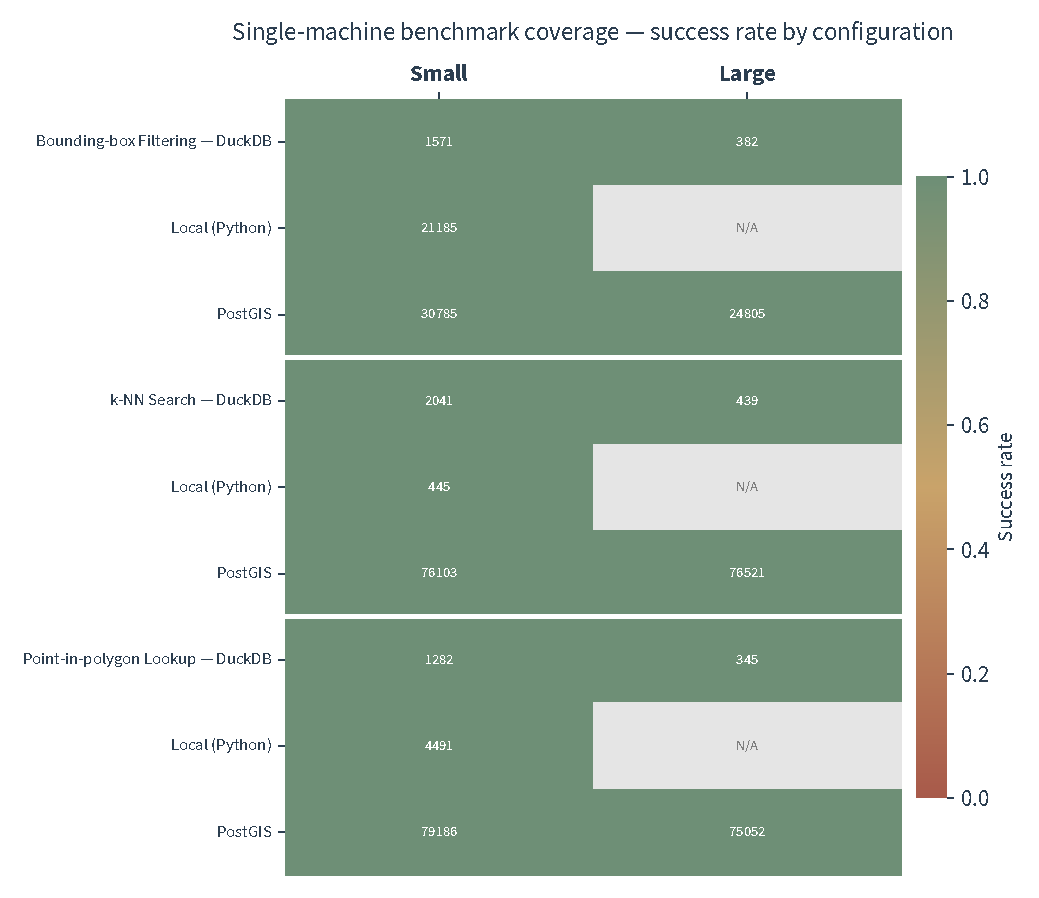
\includegraphics[width=0.85\textwidth]{Chapters/06-results/sub-chapters/figures/06-results-coverage-single-machine.pdf}
    \caption[Run-completeness coverage grid (single-machine)]{Completion status of
    every single-machine configuration across the three query patterns and the small
    and large tiers. Each cell records whether the run completed in full, completed
    partially under the sequential stopping rule, or did not run for that
    combination. Every Shapefile cell beyond the small tier is absent by design and
    is marked as did-not-run rather than as missing or failed cells.}
    \label{fig:results-coverage-single-machine}
\end{figure}

\begin{figure}[H]
    \centering
    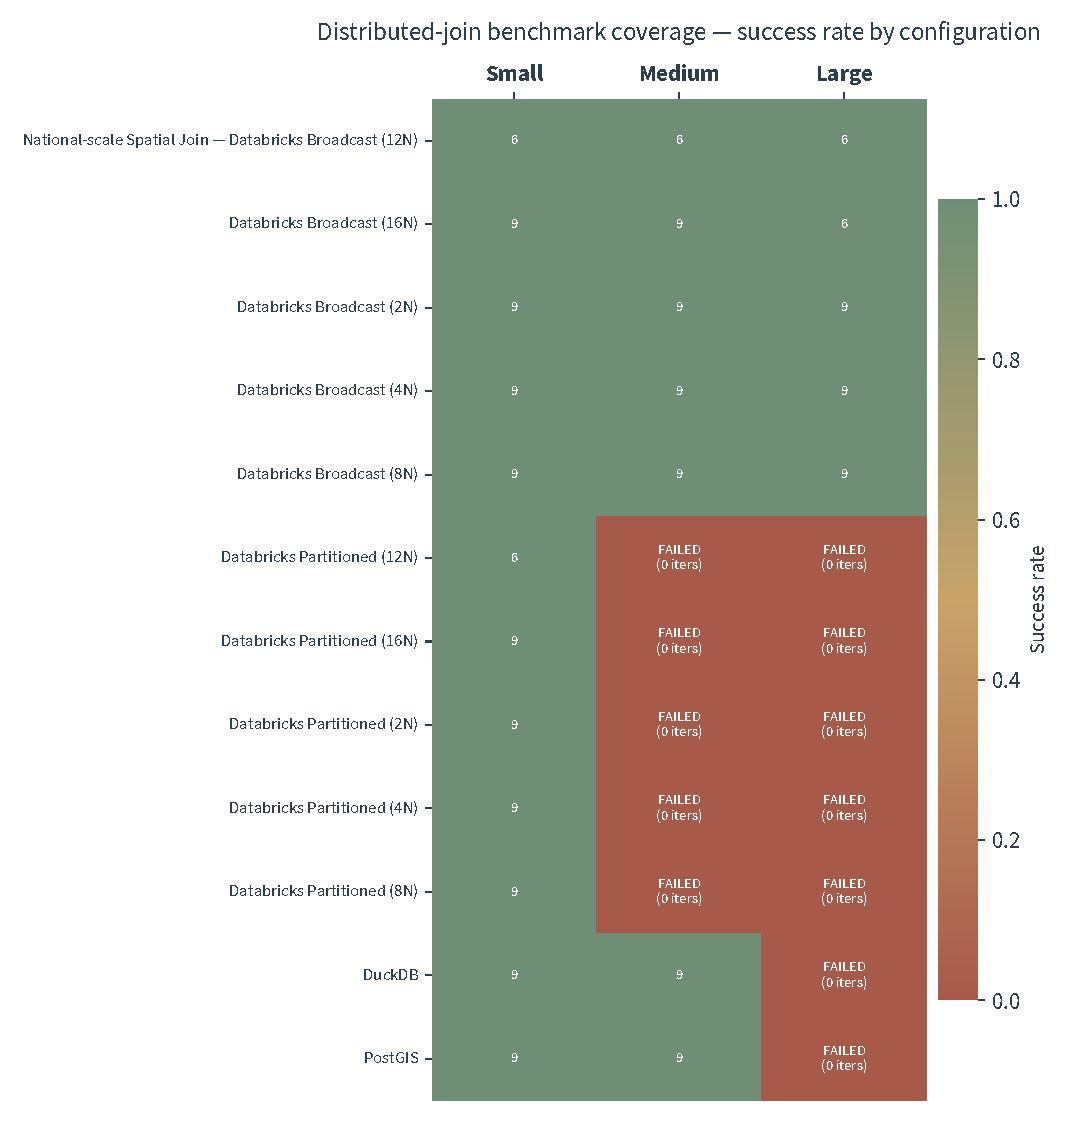
\includegraphics[width=0.85\textwidth]{Chapters/06-results/sub-chapters/figures/06-results-coverage-distributed.pdf}
    \caption[Run-completeness coverage grid (distributed join)]{Completion status of
    every configuration for the national-scale spatial join -- the single-node DuckDB
    and PostGIS engines and the Apache Sedona broadcast and partitioned variants at
    each worker count -- across the small, medium, and large tiers. Each cell records
    whether the run completed in full, completed partially, or failed or did not run
    for that combination.}
    \label{fig:results-coverage-distributed}
\end{figure}

\subsection{Timing distributions and estimator behavior}
\label{results:overview-and-measurement-quality:timing-distributions-and-estimator-behavior}

Figure~\ref{fig:results-warmup} shows the per-iteration timing behavior for a representative cell, the point-in-polygon lookup on DuckDB over GeoParquet at the small tier. The distribution in panel~(a) rises off a hard lower bound and trails a long right tail, so the mean and the median both sit above the fastest observed iteration. This one-sided, right-skewed contamination is the shape the minimum estimator is chosen to reject (Section~\ref{research-design-and-methodology:statistical-analysis:summary-statistics-and-the-choice-of-estimator}). Figure~\ref{fig:appendix-estimator-illustration} reports the quantified separation between the minimum, the median, and the mean for this same cell. Panel~(b) plots elapsed time against iteration index within a single measurement pass. The per-iteration times scatter within a narrow band above the steady-state minimum, without a pronounced warmup ramp.

\begin{figure}[H]
    \centering
    \subfloat[Per-iteration elapsed-time distribution.\label{fig:results-warmup-distribution}]{%
        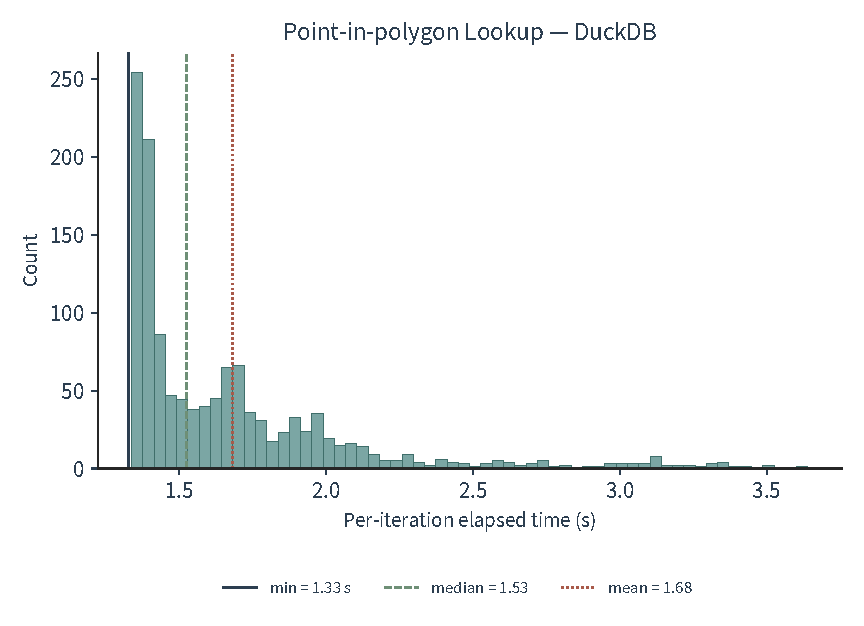
\includegraphics[valign=t, width=0.45\textwidth]{Chapters/06-results/sub-chapters/figures/06-results-warmup-distribution.pdf}}%
    \hfill
    \subfloat[Warmup-to-steady-state decay.\label{fig:results-warmup-decay}]{%
        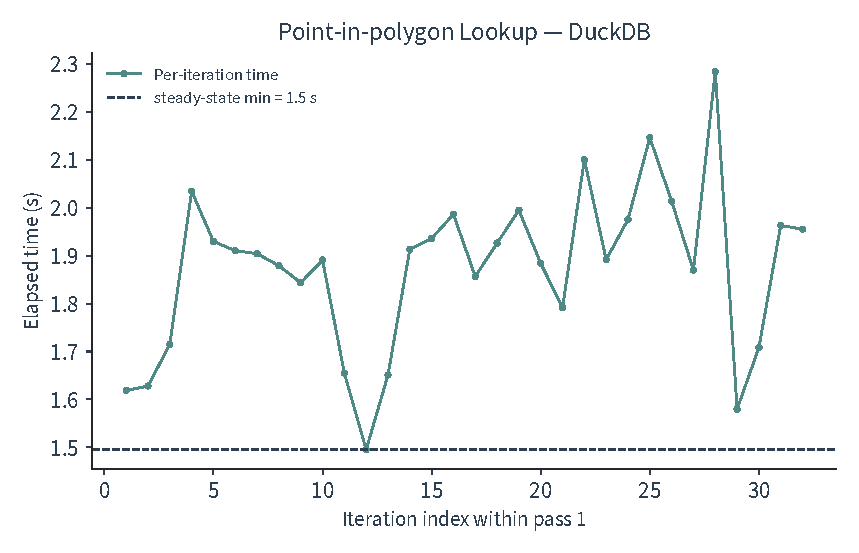
\includegraphics[valign=t, width=0.45\textwidth]{Chapters/06-results/sub-chapters/figures/06-results-warmup-decay.pdf}}%
    \caption[Per-iteration timing distribution and warmup behavior]{Per-iteration
    timing behavior for one representative configuration, workload, and tier (DuckDB
    over GeoParquet, point-in-polygon, small tier). Panel~(a) shows the distribution
    of per-iteration elapsed times, with its hard lower bound and the one-sided,
    right-skewed contamination that motivates reporting the minimum rather than the
    mean \parencite{chen2016_robust_benchmarking_noisy_environments}. Panel~(b) shows
    per-iteration elapsed time against iteration index within one measurement pass,
    fluctuating within a narrow band above the steady-state minimum (dashed).}
    \label{fig:results-warmup}
\end{figure}

\subsection{Iteration counts and convergence}
\label{results:overview-and-measurement-quality:iteration-counts-and-convergence}

Figure~\ref{fig:results-convergence} traces the sequential stopping rule for the same representative cell over a single measurement pass. The running half-width of the bootstrap confidence interval, expressed as a fraction of the running minimum, reaches the \num{5}\% relative target within the first iterations and stays close to it thereafter.

Table~\ref{tab:results-achieved-n} reports, for each single-machine cell, the achieved count of successful iterations, the minimum-estimator elapsed time, the final confidence-interval half-width, and the recorded stop reason. Every cell that ran reached the precision target rather than a budget or timeout limit. The achieved counts ranged across cells from \num{345} iterations for the point-in-polygon lookup on DuckDB at the large tier to \num{79186} for the same pattern on PostGIS at the small tier. The national-scale join took the fixed-iteration branch of the protocol rather than the sequential rule (Section~\ref{research-design-and-methodology:workloads:iteration-counts}), so its per-cell counts are reported with the distributed results in Table~\ref{tab:distributed-join-descriptive-statistics}.

\begin{figure}[H]
    \centering
    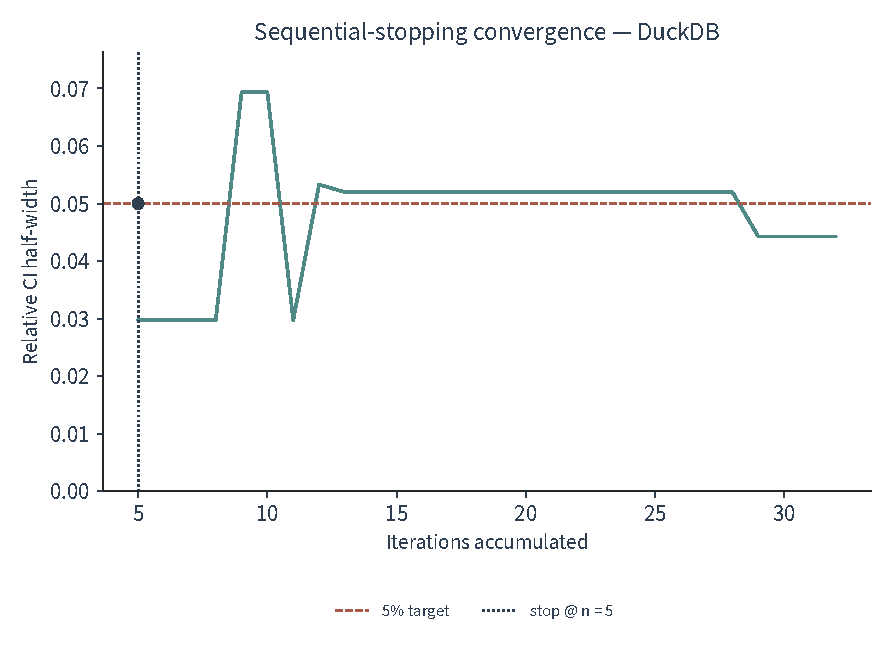
\includegraphics[width=0.7\textwidth]{Chapters/06-results/sub-chapters/figures/06-results-convergence.pdf}
    \caption[Sequential-stopping convergence]{Convergence of the sequential stopping
    rule for one representative configuration, workload, and tier (DuckDB over
    GeoParquet, point-in-polygon, small tier), over a single measurement pass. The
    running bootstrap \num{95}\% confidence-interval half-width, expressed as a
    fraction of the running minimum elapsed time, is plotted against the number of
    accumulated iterations; the horizontal line marks the \num{5}\% relative target
    half-width \parencite{georges2007_statistically_rigorous_java_performance,laaber2019_software_microbenchmarking_cloud},
    and the marker indicates the first iteration at which the running half-width meets
    that target.}
    \label{fig:results-convergence}
\end{figure}

\begin{table}[H]
    \centering
    \footnotesize
    \setlength{\tabcolsep}{6pt}
    \renewcommand{\arraystretch}{1.2}
    \resizebox{\textwidth}{!}{%
    \begin{tabular}{@{}l l l r r r l@{}}
        \toprule
        \textbf{Configuration} & \textbf{Workload} & \textbf{Tier} & \textbf{Achieved $n$} & \textbf{Min.\ (\si{\second})} & \textbf{\acrshort{ci} half-width} & \textbf{Stop reason} \\
        \midrule
        \inputtablebody{Chapters/06-results/sub-chapters/tables/06-achieved-iterations.tex}
        \bottomrule
    \end{tabular}}
    \caption[Achieved iteration counts and convergence]{Achieved count of successful
    timed iterations, minimum-estimator elapsed time, final bootstrap \num{95}\%
    confidence-interval half-width, and recorded stop reason for each single-machine
    configuration, query pattern, and size tier. The reported $n$ is the achieved
    number of successful iterations recorded in the run metadata, not the configured
    ceiling. Cells that did not run by design carry an explicit did-not-run stop
    reason rather than a zero count.}
    \label{tab:results-achieved-n}
\end{table}
\section{Single-machine query performance (RQ1)}
\label{results:single-machine-query-performance}

% ORIENTING COMMENT (section intro prose -- TODO below). One paragraph, no
%   numbers: present the single-node configurations -- DuckDB over GeoParquet,
%   PostGIS, and GeoPandas over Shapefile (small tier only) -- compared
%   descriptively across the three outcome dimensions in order: data transferred,
%   then wall-clock time, then operational cost. Results only; interpretation is
%   deferred to the Discussion (Chapter~\ref{ch:discussion}).
% GRID RULE (every grid figure in this section): the kNN workload ran at the
%   small tier only, and the Shapefile configuration ran at the small tier only;
%   leave those slots as did-not-run-by-design. Do not draw an empty bar, a zero,
%   or any marker that would imply a missing or failed cell.

% TODO (prose): section-opening paragraph per the orienting comment above.

\subsection{Data transferred}
\label{results:single-machine-query-performance:data-transferred}

% TODO (prose): factual readout only of the bytes-transferred results -- magnitudes
% and orderings per cell, with CIs. Refer to
% Figure~\ref{fig:single-machine-bytes-transferred} and, optionally,
% Figure~\ref{fig:single-machine-bytes-vs-time}. No interpretation (-> Discussion).

\begin{figure}[H]
    \centering
    % WHAT IT SHOWS: bytes-transferred grid. Rows = workload pattern, columns =
    %   size tier. Within each cell, grouped bars per configuration on a
    %   logarithmic y-axis with bootstrap confidence-interval whiskers. Bytes
    %   received and bytes sent shown separately (two grids or two panels).
    % CAPTION MUST STATE: the grid layout (pattern x tier); log y-axis; that
    %   whiskers are bootstrap CIs; that received and sent are separated; the
    %   estimator (median for transfer metrics, per the methodology).
    % ANNOTATE: Shapefile is read from the LOCAL filesystem, so its network bytes
    %   are ~0; label this explicitly so the near-zero bar is not misread as a
    %   missing cell. Leave the Shapefile-beyond-small and kNN-large slots as
    %   did-not-run-by-design.
    % DESCRIPTIVE ONLY: report the bars; no interpretation (-> Discussion).
    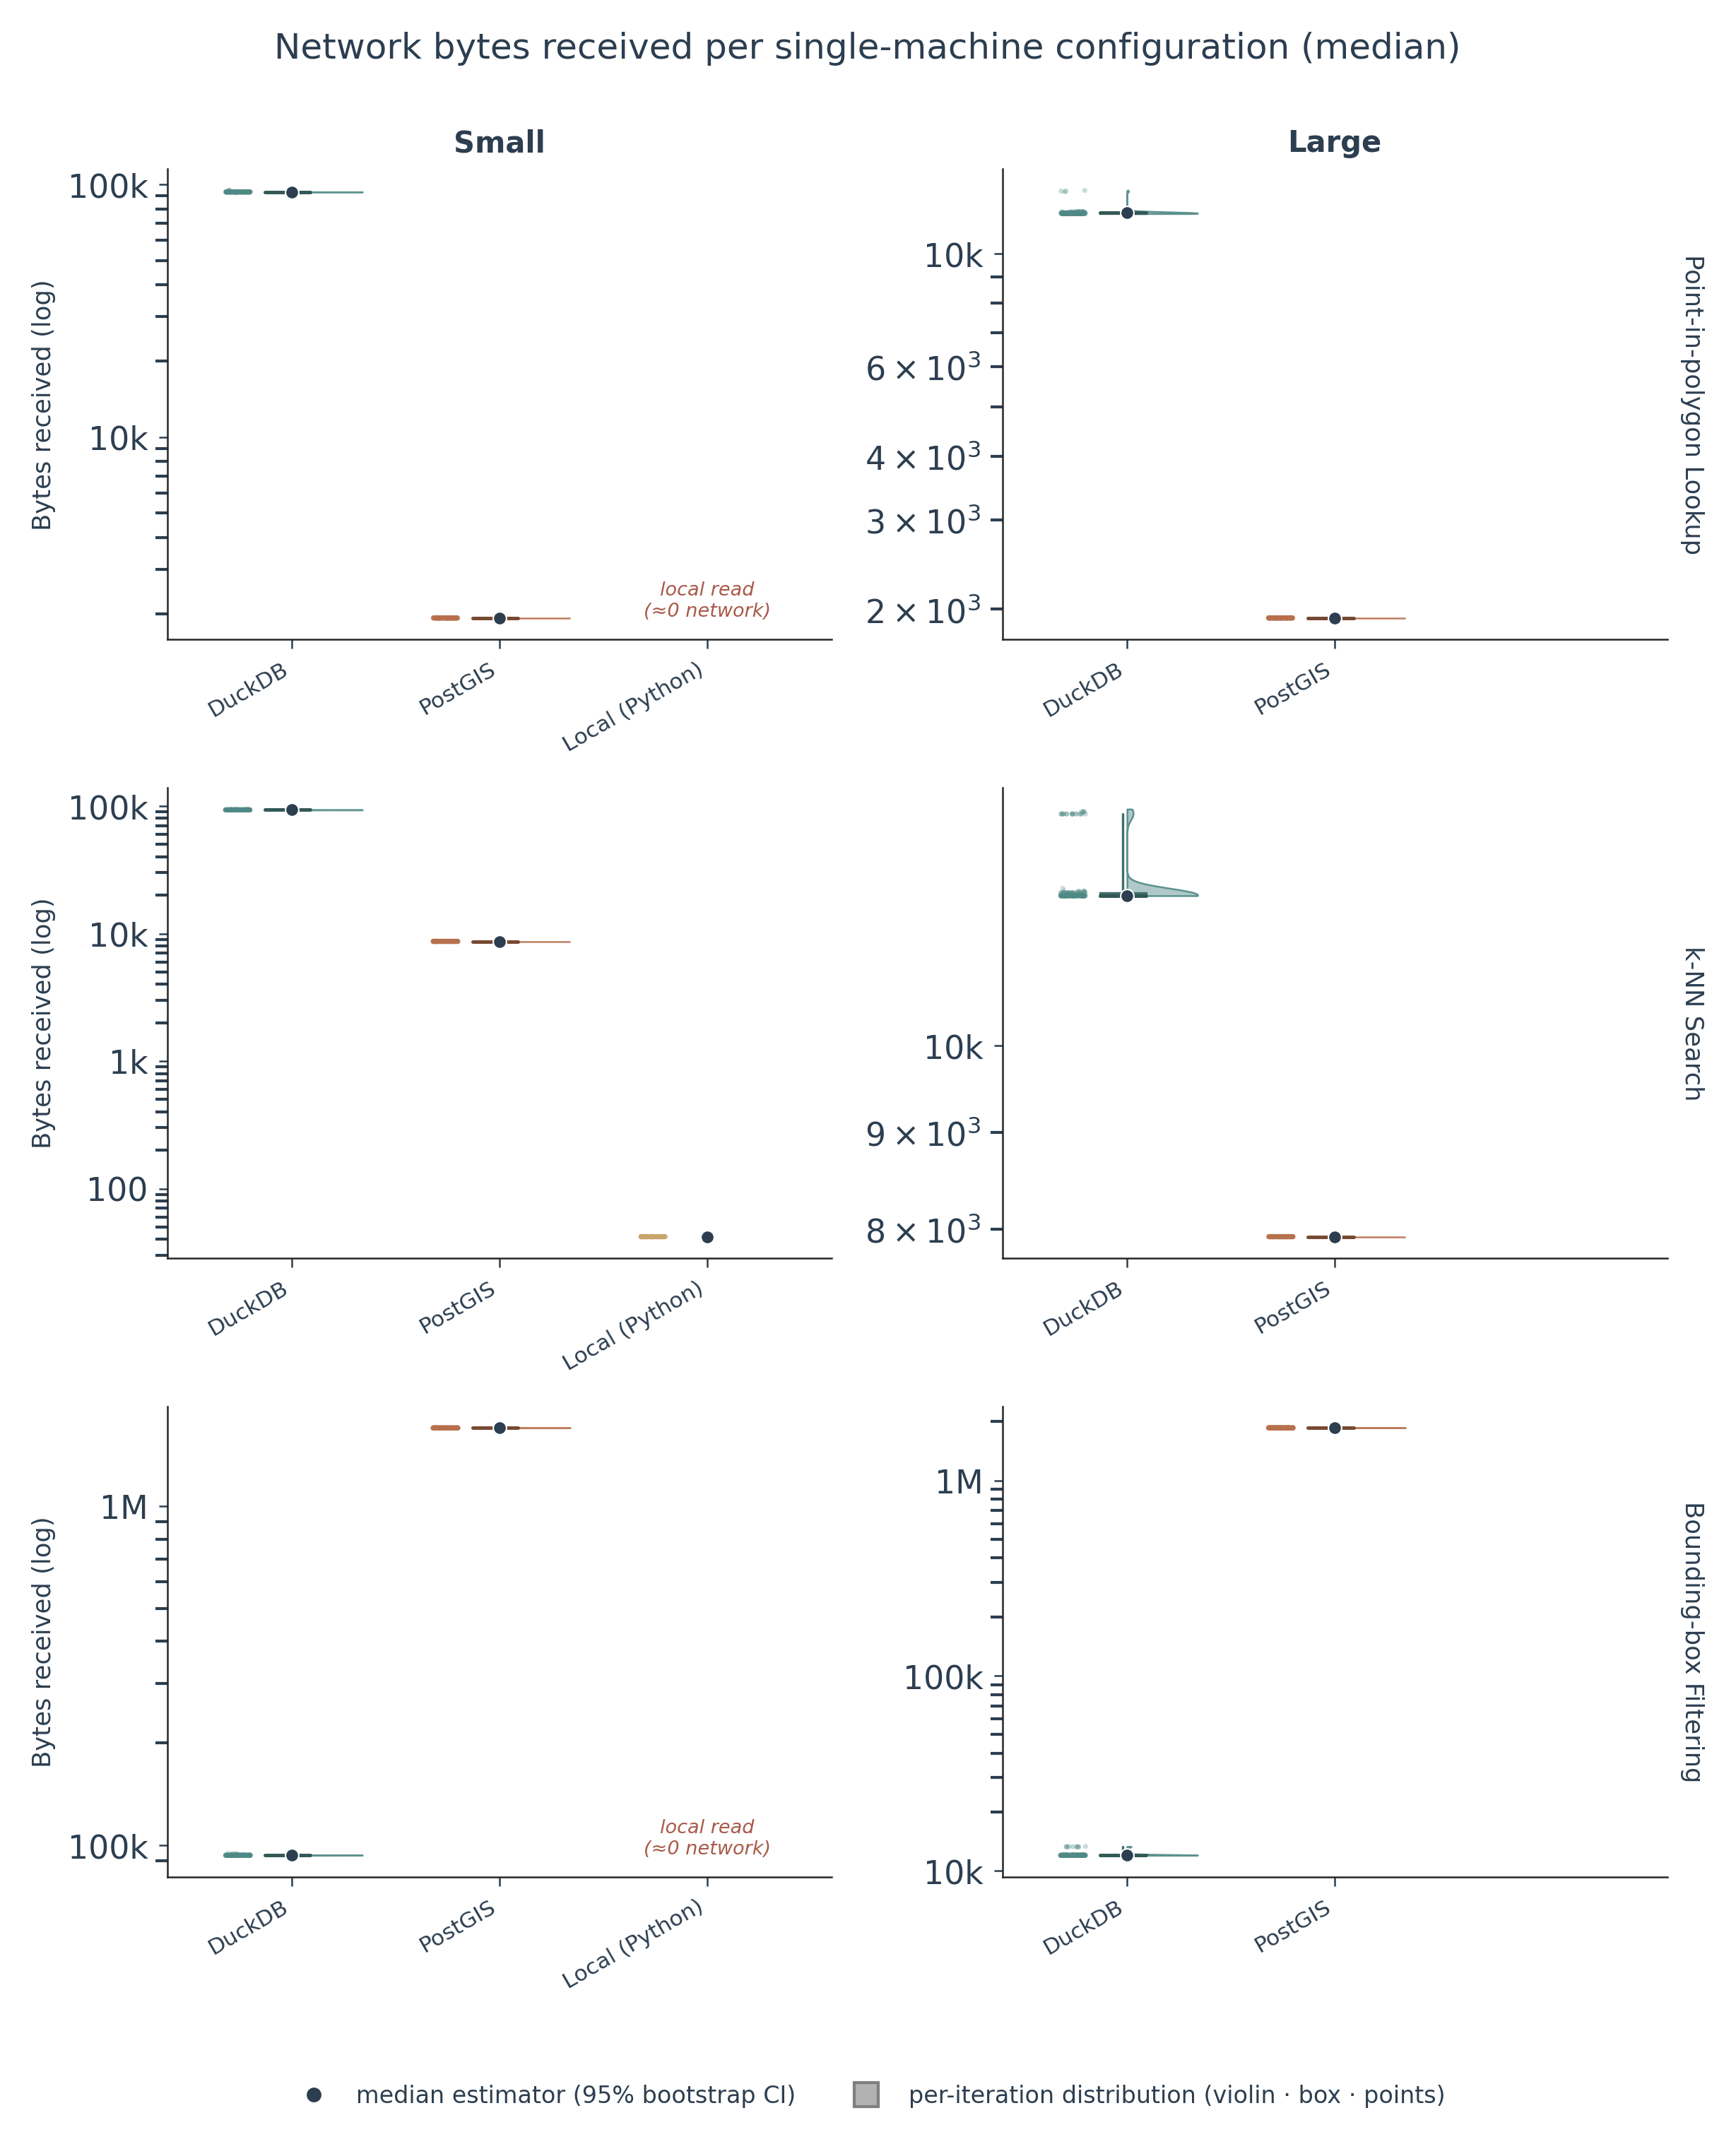
\includegraphics[width=0.95\textwidth]{Chapters/06-results/sub-chapters/figures/06-single-machine-bytes-transferred.png}
    \caption[Data transferred per single-machine configuration]{Bytes transferred
    by each single-machine configuration, arranged as a grid with workload
    patterns in rows and size tiers in columns. Within each cell, bars give the
    per-configuration volume on a logarithmic axis with bootstrap
    confidence-interval whiskers; bytes received and bytes sent are shown
    separately. The Shapefile configuration reads from the local filesystem, so
    its network transfer is approximately zero and is labelled as such rather than
    left blank. Bar colour encodes configuration using the thesis palette.}
    \label{fig:single-machine-bytes-transferred}
\end{figure}

\begin{figure}[H]
    \centering
    % OPTIONAL supplementary float (not required by the chapter outline; keep or
    %   drop). WHAT IT SHOWS: scatter of bytes transferred against wall-clock time,
    %   one point per configuration x pattern x tier, exposing the transfer-vs-time
    %   relationship; logarithmic axes; point colour by configuration.
    % CAPTION MUST STATE: the two axes and that each point is one cell.
    % DESCRIPTIVE ONLY.
    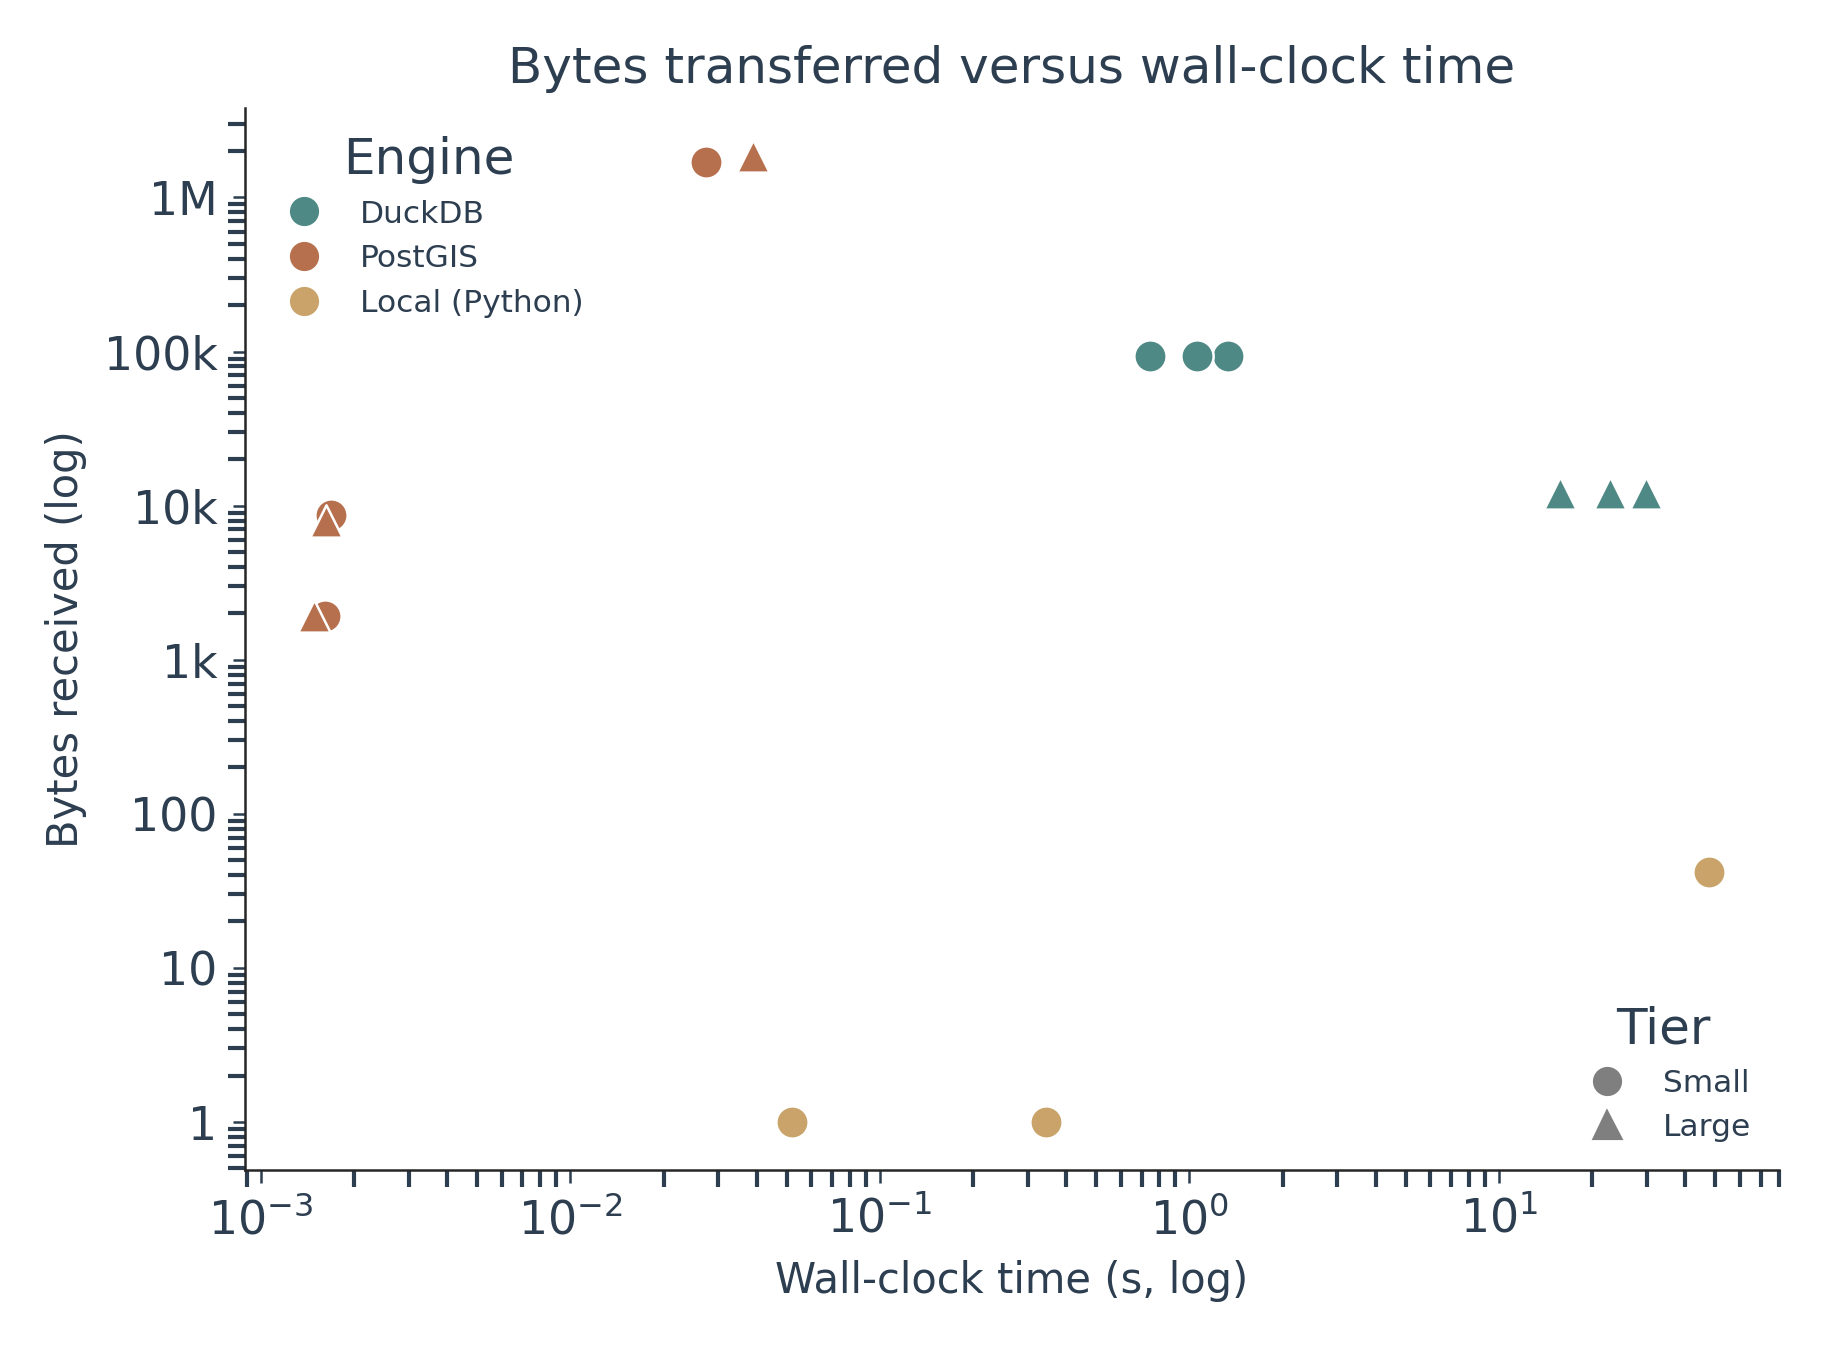
\includegraphics[width=0.7\textwidth]{Chapters/06-results/sub-chapters/figures/06-single-machine-bytes-vs-time.png}
    \caption[Bytes transferred versus wall-clock time]{Relationship between bytes
    transferred and wall-clock time across single-machine configurations, with one
    point per configuration, workload pattern, and size tier on logarithmic axes.
    Point colour encodes configuration using the thesis palette.}
    \label{fig:single-machine-bytes-vs-time}
\end{figure}

\subsection{Wall-clock time}
\label{results:single-machine-query-performance:wall-clock-time}

% TODO (prose): factual readout only of the wall-clock-time results. Refer to
% Figure~\ref{fig:single-machine-wall-clock-time}. No interpretation (-> Discussion).

\begin{figure}[H]
    \centering
    % WHAT IT SHOWS: wall-clock-time grid, SAME layout as the bytes grid
    %   (Figure~\ref{fig:single-machine-bytes-transferred}): rows = pattern,
    %   columns = tier, grouped bars per configuration, logarithmic y-axis,
    %   bootstrap confidence-interval whiskers.
    % CAPTION MUST STATE: the grid layout; that the bar height is the MINIMUM
    %   estimator (per the methodology); log y-axis; bootstrap CI whiskers.
    % Leave the Shapefile-beyond-small and kNN-large slots as did-not-run-by-design.
    % DESCRIPTIVE ONLY: report the bars; no interpretation (-> Discussion).
    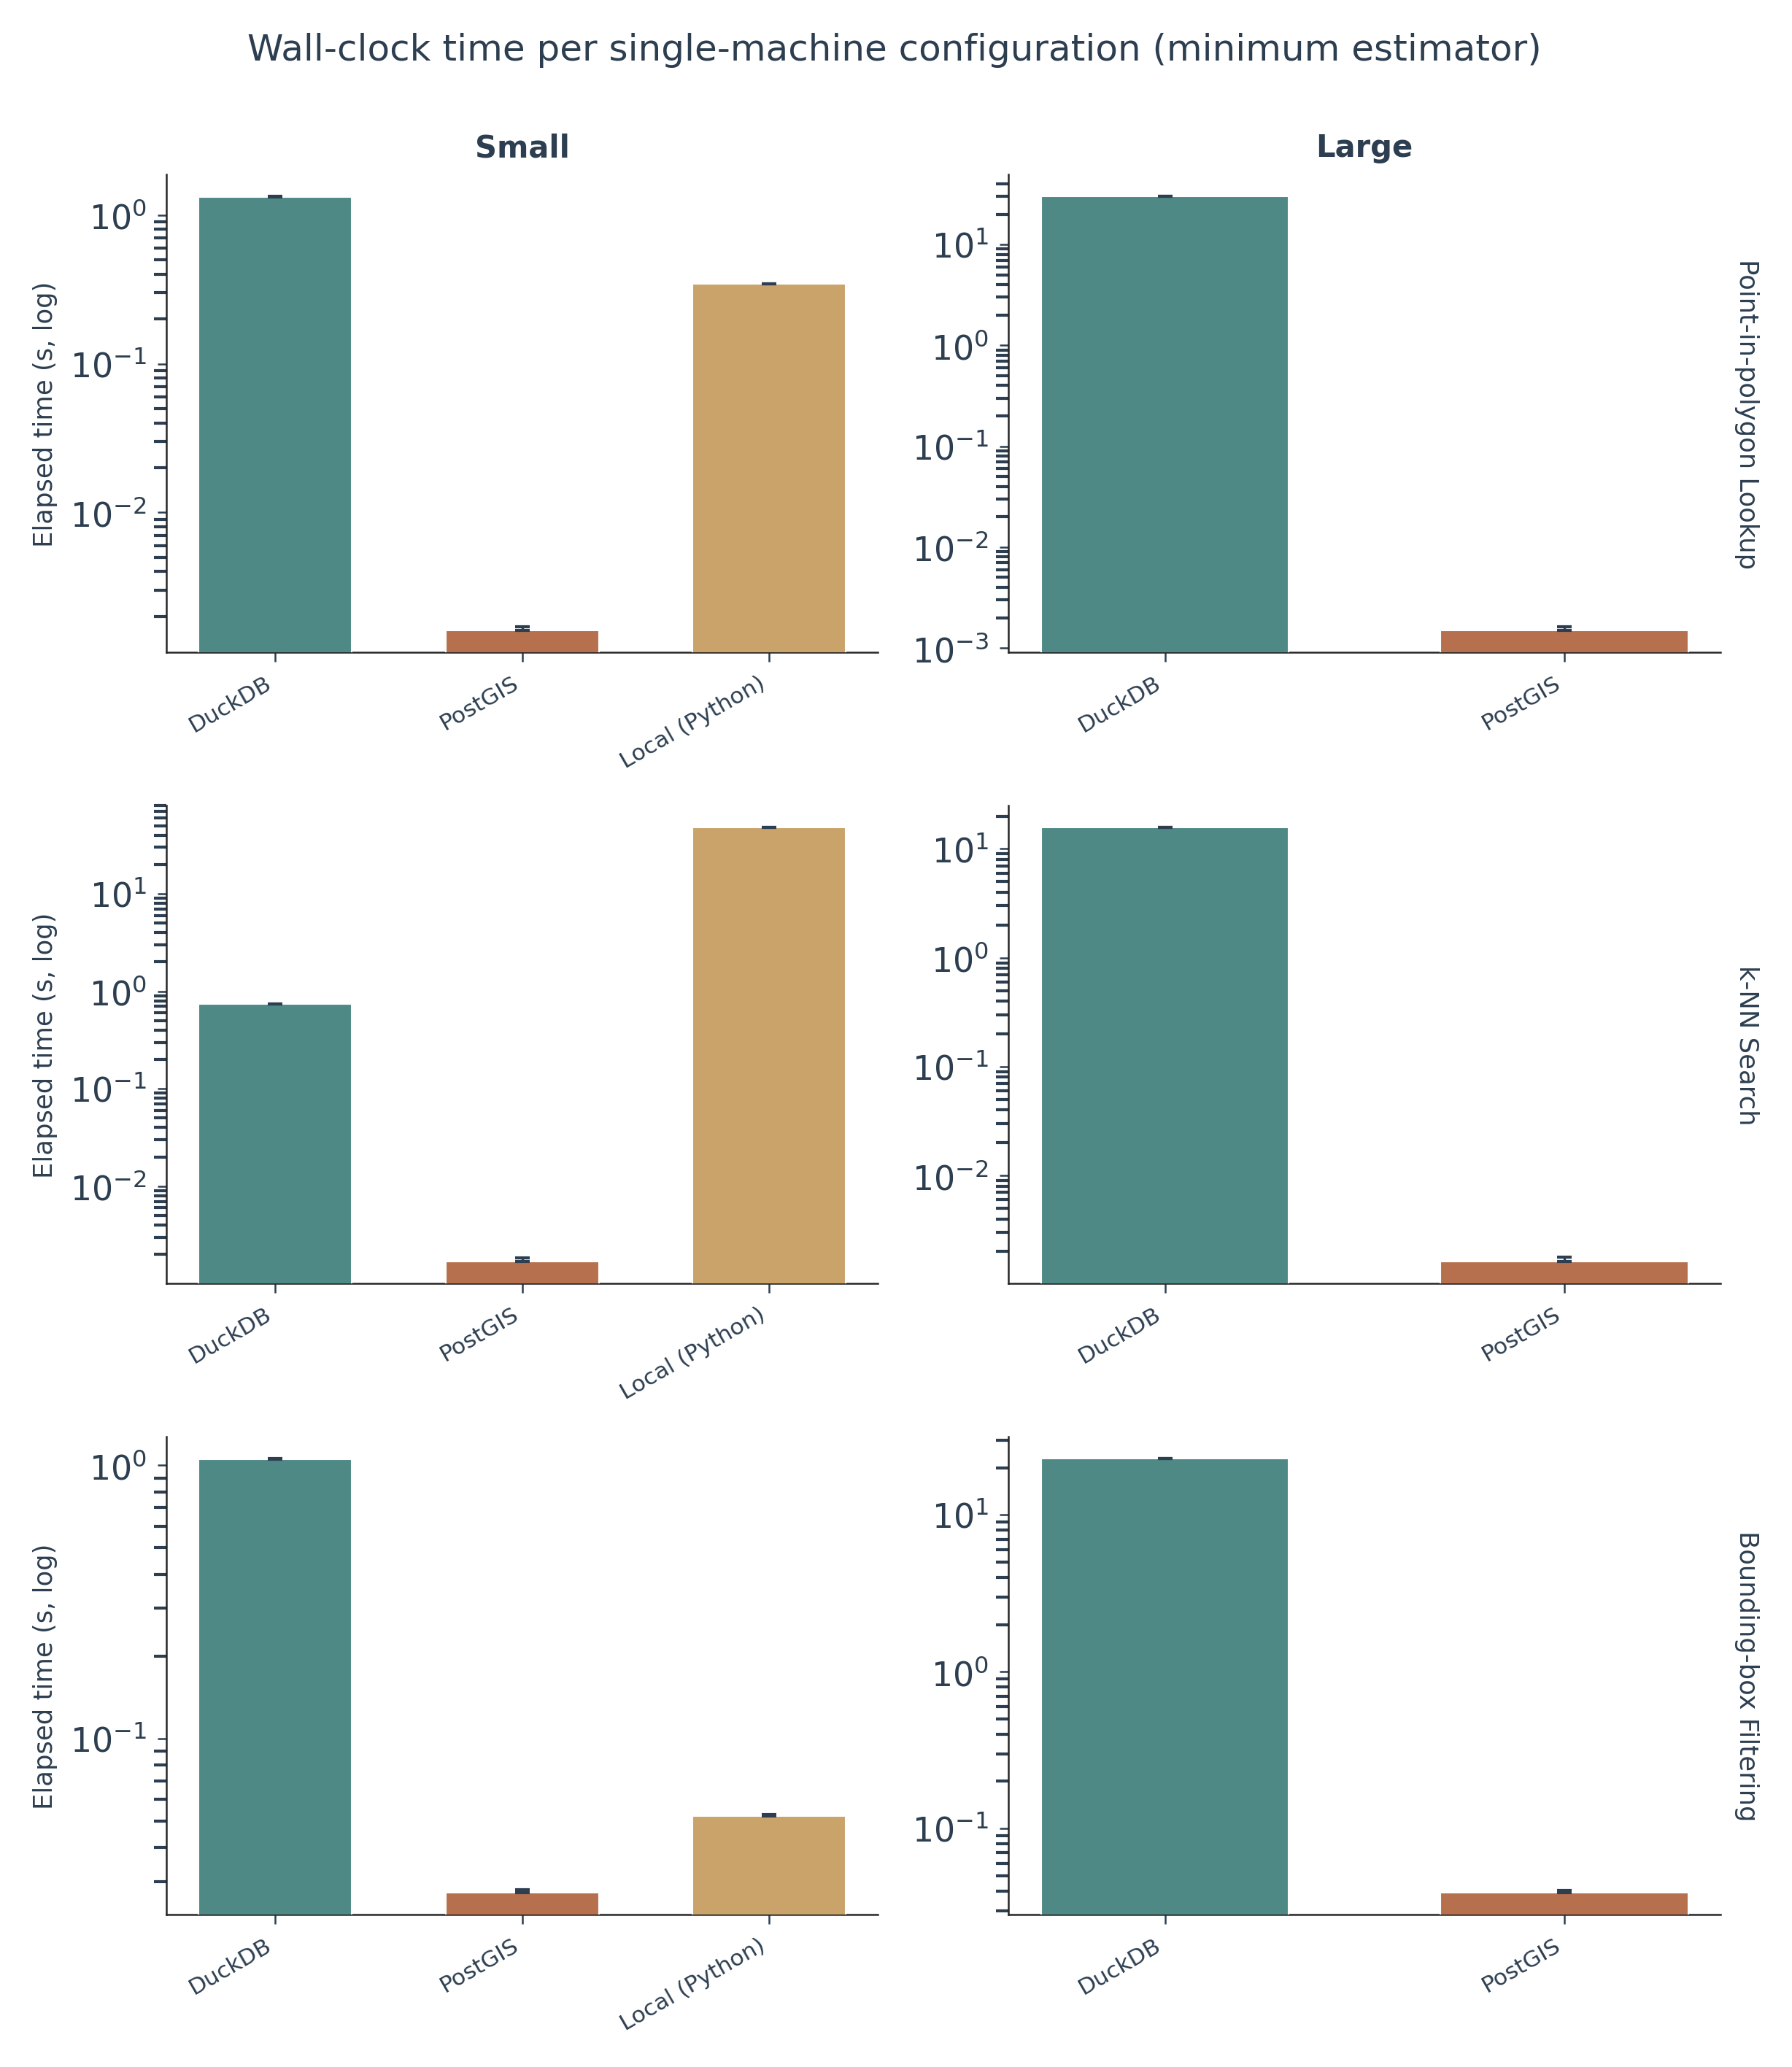
\includegraphics[width=0.95\textwidth]{Chapters/06-results/sub-chapters/figures/06-single-machine-wall-clock-time.png}
    \caption[Wall-clock time per single-machine configuration]{Wall-clock time of
    each single-machine configuration, in the same grid layout as the
    bytes-transferred figure: workload patterns in rows, size tiers in columns.
    Bar height is the minimum-estimator elapsed time on a logarithmic axis with
    bootstrap confidence-interval whiskers. Bar colour encodes configuration using
    the thesis palette.}
    \label{fig:single-machine-wall-clock-time}
\end{figure}

\subsection{Operational cost}
\label{results:single-machine-query-performance:operational-cost}

% TODO (prose): factual readout only of the operational-cost results, broken into
% the four cost terms. Refer to Figure~\ref{fig:single-machine-operational-cost}.
% No interpretation (-> Discussion).

\begin{figure}[H]
    \centering
    % WHAT IT SHOWS: stacked operational-cost bars, one bar per configuration,
    %   faceted by workload pattern. Each bar is stacked into the FOUR cost terms
    %   of the cost model: compute, storage, operations, and egress.
    % CAPTION MUST STATE: that cost is decomposed into the four model terms --
    %   compute, storage, operations, egress -- and name their source (the
    %   four-term cost model and unit-price table of the methodology). Note that a
    %   single-node engine reading from object storage draws all four terms,
    %   whereas the local-filesystem Shapefile path draws no operations/egress.
    % NOTE: the prior draft showed only two terms (compute + transfer); the real
    %   model is four-term -- see
    %   Section~\ref{research-design-and-methodology:metrics-and-cost-model:cost-model}
    %   and the rates in Table~\ref{tab:cost-model-unit-prices}.
    % Leave the Shapefile-beyond-small and kNN-large slots as did-not-run-by-design.
    % DESCRIPTIVE ONLY: report the stacks; no interpretation (-> Discussion).
    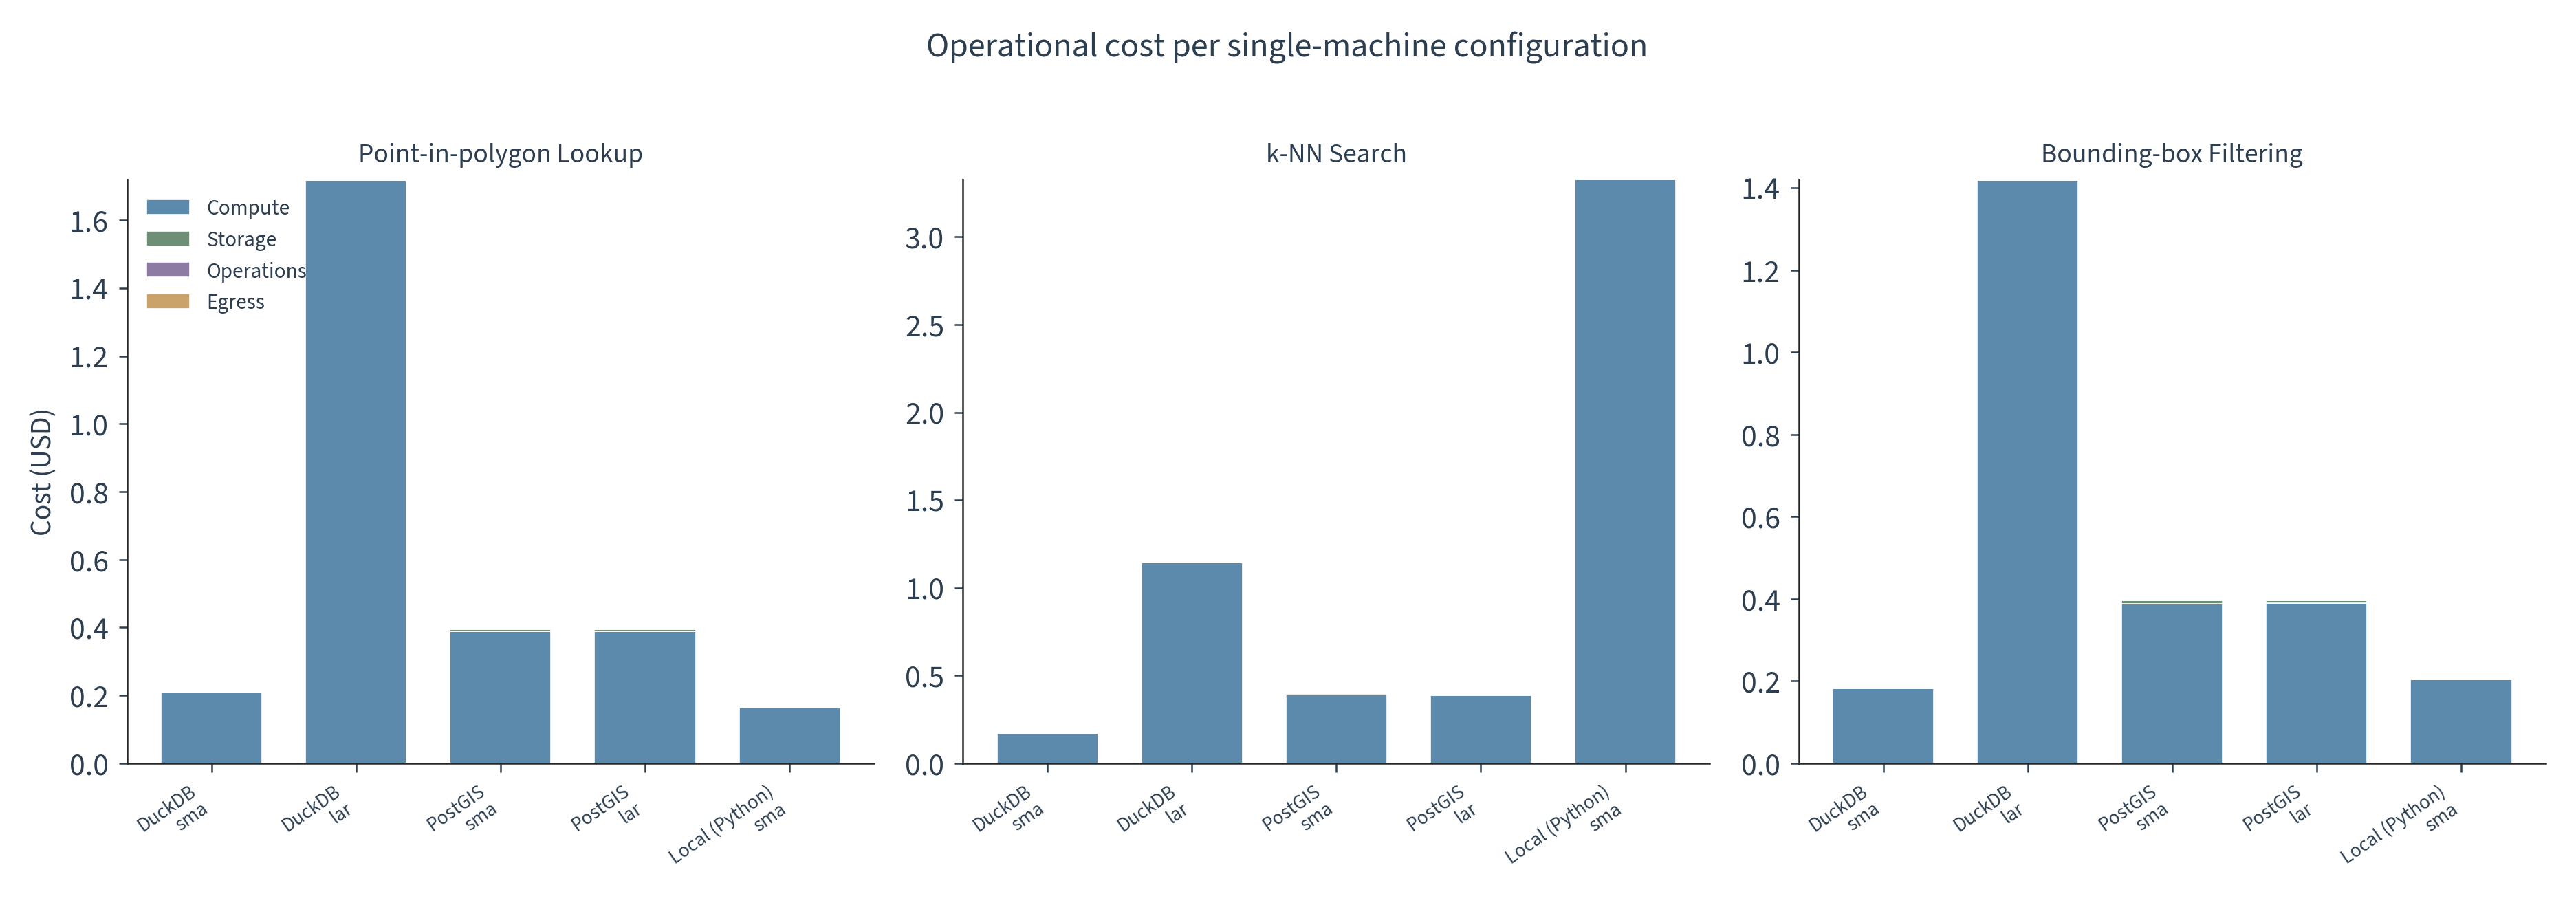
\includegraphics[width=0.9\textwidth]{Chapters/06-results/sub-chapters/figures/06-single-machine-operational-cost.png}
    \caption[Operational cost per single-machine configuration]{Operational cost
    of each single-machine configuration, faceted by workload pattern. Each bar is
    stacked into the four terms of the cost model -- compute, storage, operations,
    and egress -- whose definitions and unit prices are given in
    Section~\ref{research-design-and-methodology:metrics-and-cost-model:cost-model}
    and Table~\ref{tab:cost-model-unit-prices}. Term colour uses the thesis
    palette.}
    \label{fig:single-machine-operational-cost}
\end{figure}

\section{Distributed join and scaling (RQ2)}
\label{results:distributed-join-and-scaling}

% ORIENTING COMMENT (section intro prose -- TODO below). One paragraph, no
%   numbers: present the national-scale spatial join run on Apache Sedona
%   (Databricks) across worker counts {2, 4, 8, 12, 16} and the two execution
%   strategies (broadcast and partitioned), against the single-node PostGIS and
%   DuckDB baselines, at the small/medium/large tiers. Present, in order: scaling
%   behavior, absolute performance vs. the single-node baselines, the
%   execution-phase breakdown, then cost and the cost-time tradeoff. Results only;
%   interpretation is deferred to the Discussion (Chapter~\ref{ch:discussion}).

% TODO (prose): section-opening paragraph per the orienting comment above.

\subsection{Scaling behavior}
\label{results:distributed-join-and-scaling:scaling-behavior}

% TODO (prose): factual readout only of speedup and parallel efficiency -- the
% curve shapes and where they depart from ideal. Refer to
% Figure~\ref{fig:distributed-speedup-efficiency}. No interpretation (-> Discussion).

\begin{figure}[H]
    \centering
    % WHAT IT SHOWS: two-panel scaling float over worker counts {2, 4, 8, 12, 16}.
    %   (a) speedup S(n) = T_2 / T_n, one series for broadcast and one for
    %       partitioned, with an ideal-linear reference S(n) = n/2 (baseline is
    %       the 2-worker cluster).
    %   (b) paired parallel efficiency E(n) = (2/n) * S(n), same two series, with
    %       the ideal E(n) = 1 reference.
    % CAPTION MUST STATE: the worker-count axis; that speedup and efficiency are
    %   defined relative to the 2-worker baseline (n0 = 2) per
    %   Equation~\ref{eq:speedup-parallel-efficiency}; the two strategies; and the
    %   ideal reference in each panel.
    % DESCRIPTIVE ONLY: report the curves; no interpretation (-> Discussion).
    \subfloat[Speedup $S(n)$.\label{fig:distributed-speedup}]{%
        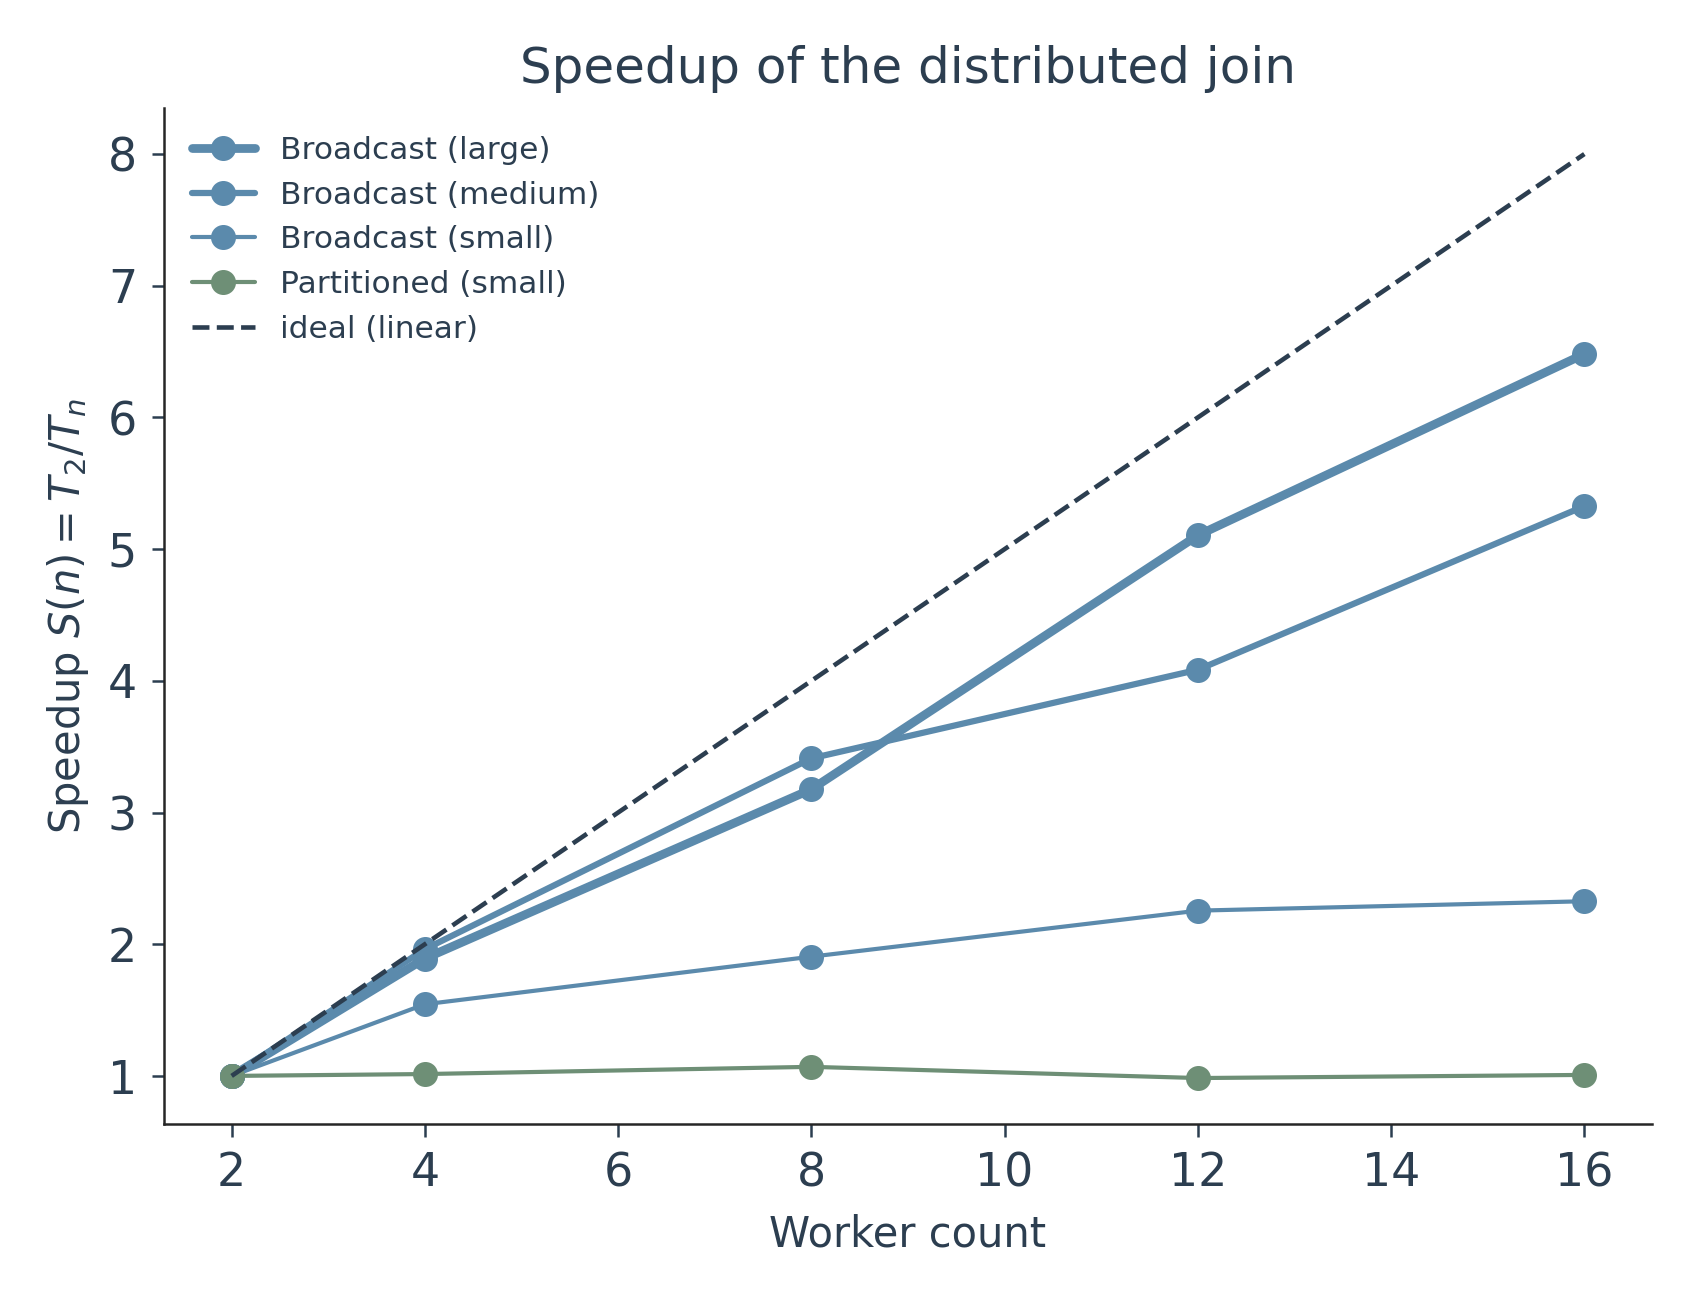
\includegraphics[valign=t, width=0.45\textwidth]{Chapters/06-results/sub-chapters/figures/06-distributed-speedup.png}}%
    \hfill
    \subfloat[Parallel efficiency $E(n)$.\label{fig:distributed-efficiency}]{%
        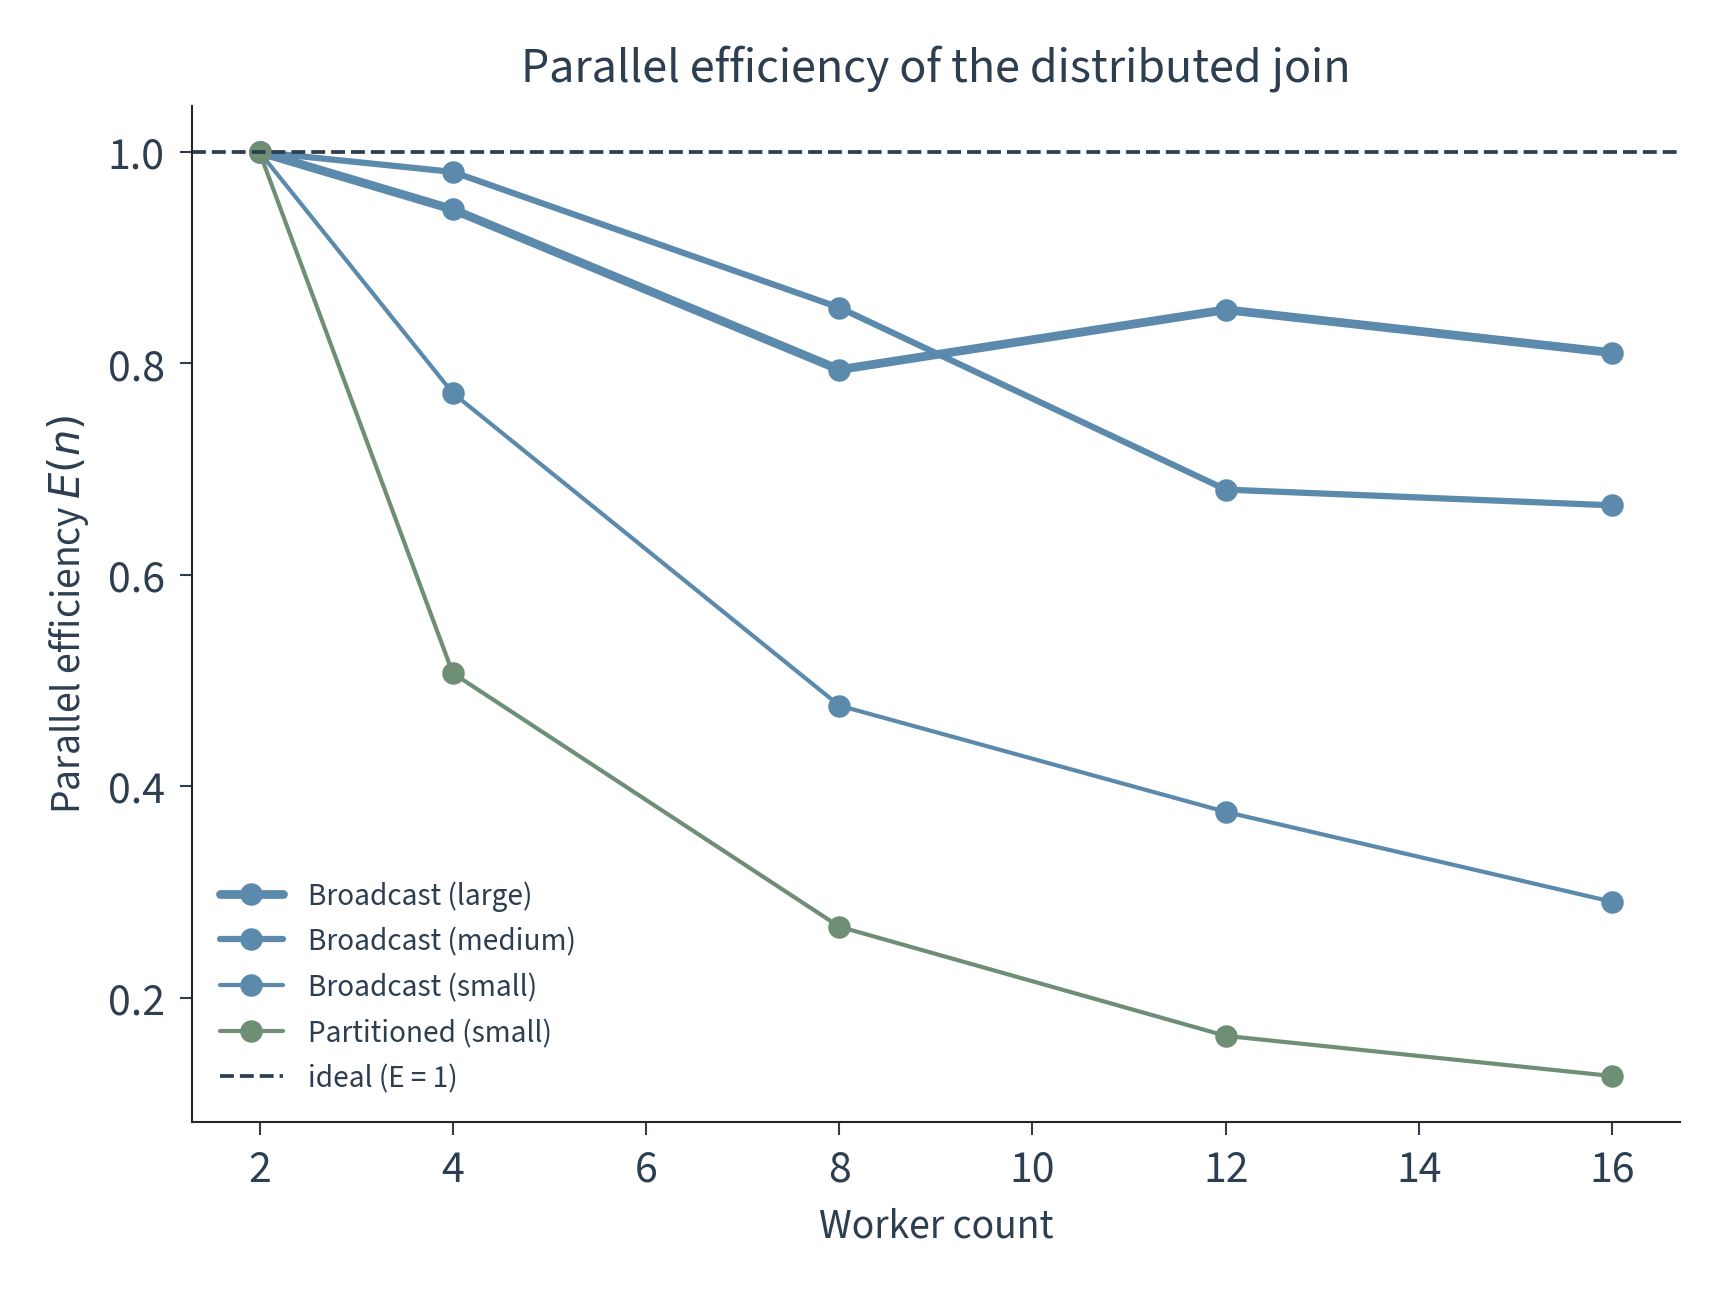
\includegraphics[valign=t, width=0.45\textwidth]{Chapters/06-results/sub-chapters/figures/06-distributed-efficiency.png}}%
    \caption[Speedup and parallel efficiency of the distributed join]{Scaling of
    the distributed spatial join over worker counts $\{2, 4, 8, 12, 16\}$, defined
    relative to the two-worker baseline ($n_0 = 2$) of
    Equation~\ref{eq:speedup-parallel-efficiency}. Panel~(a) shows speedup
    $S(n) = T_2/T_n$ for the broadcast and partitioned strategies against an
    ideal-linear reference; panel~(b) shows the paired parallel efficiency
    $E(n) = (2/n)\,S(n)$ against its ideal of one. Series colour encodes join
    strategy and the reference line uses a neutral palette colour.}
    \label{fig:distributed-speedup-efficiency}
\end{figure}

\subsection{Absolute performance vs. single-node baselines}
\label{results:distributed-join-and-scaling:absolute-performance-vs-single-node-baselines}

% TODO (prose): factual readout only -- absolute wall-clock at each worker count
% against the PostGIS and DuckDB baselines, and the worker count (if any, within
% 2--16) at which the distributed join first overtakes the best single-node
% engine. Refer to Figure~\ref{fig:distributed-wall-clock-vs-workers}. No
% interpretation (-> Discussion).

\begin{figure}[H]
    \centering
    % WHAT IT SHOWS: wall-clock time (minimum estimator) against worker count
    %   {2, 4, 8, 12, 16} for the distributed join, with the single-node PostGIS
    %   and DuckDB baselines drawn as horizontal reference lines, and the crossover
    %   point -- where the distributed curve first drops below the best single-node
    %   baseline -- explicitly marked (or stated as "no crossover within 2--16").
    % CAPTION MUST STATE: the axes; that baselines are horizontal single-node
    %   reference lines; that the crossover is marked; the tier shown; the
    %   estimator.
    % STRATEGY: treat the broadcast/partitioned dimension consistently -- either
    %   plot both strategies, or pick the winning strategy and SAY SO in the
    %   caption. Keep this choice consistent with the speedup figure.
    % DESCRIPTIVE ONLY: report the crossover location; no interpretation.
    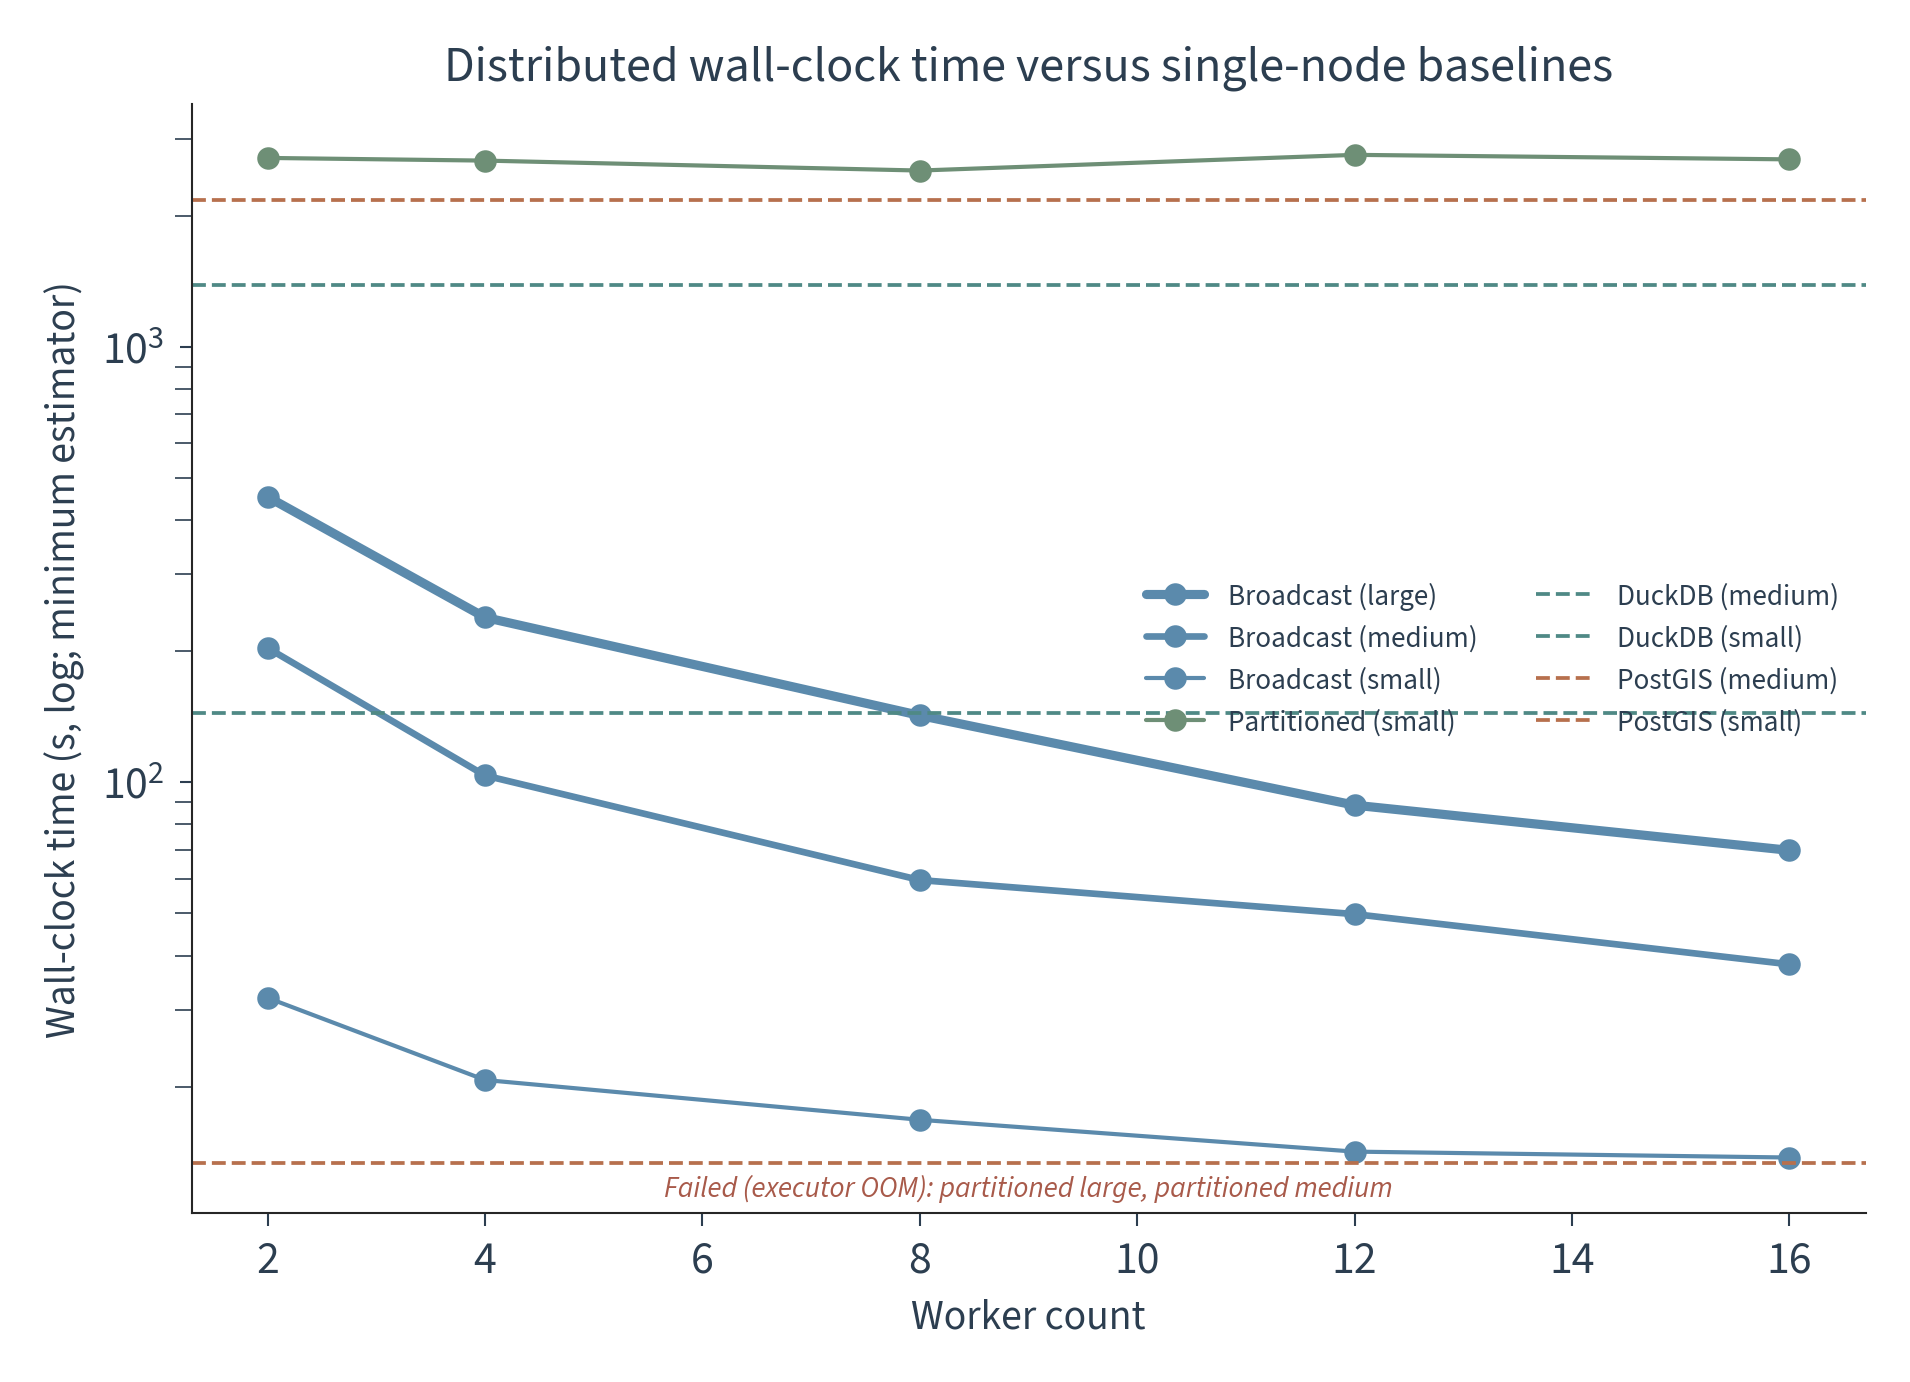
\includegraphics[width=0.8\textwidth]{Chapters/06-results/sub-chapters/figures/06-distributed-wall-clock-vs-workers.png}
    \caption[Distributed wall-clock time versus single-node baselines]{Wall-clock
    time of the distributed join as a function of worker count, with the
    single-node PostGIS and DuckDB baselines shown as horizontal reference lines.
    The worker count at which the distributed join first overtakes the best
    single-node baseline is marked as the crossover point. Bar/line height is the
    minimum-estimator elapsed time; the join strategy shown is stated consistently
    with the scaling figure.}
    \label{fig:distributed-wall-clock-vs-workers}
\end{figure}

\subsection{Execution-phase breakdown}
\label{results:distributed-join-and-scaling:execution-phase-breakdown}

% TODO (prose): factual readout only of where the distributed time and bytes go
% across phases, vs. worker count. Refer to
% Figure~\ref{fig:distributed-execution-phase-breakdown}. No interpretation.

\begin{figure}[H]
    \centering
    % WHAT IT SHOWS: two-panel execution-phase breakdown vs. worker count, using
    %   the three phases of the distributed lifecycle as instrumented
    %   (Section~\ref{research-design-and-methodology:metrics-and-cost-model:distributed-phase-metrics}):
    %   executor read time, shuffle, and driver collection.
    %   (a) stacked wall-clock time across executor-read / shuffle / driver-collection,
    %       per worker count (and strategy);
    %   (b) shuffle bytes across the same worker counts (and strategy).
    % CAPTION MUST STATE: the three phases by their instrumented names
    %   (executor read time, shuffle, driver collection -- driver collection is the
    %   clamped residual); the axes; that panel (b) is shuffle bytes.
    % DESCRIPTIVE ONLY: report the stacks; no interpretation (-> Discussion).
    \subfloat[Wall-clock time by phase.\label{fig:distributed-phase-time}]{%
        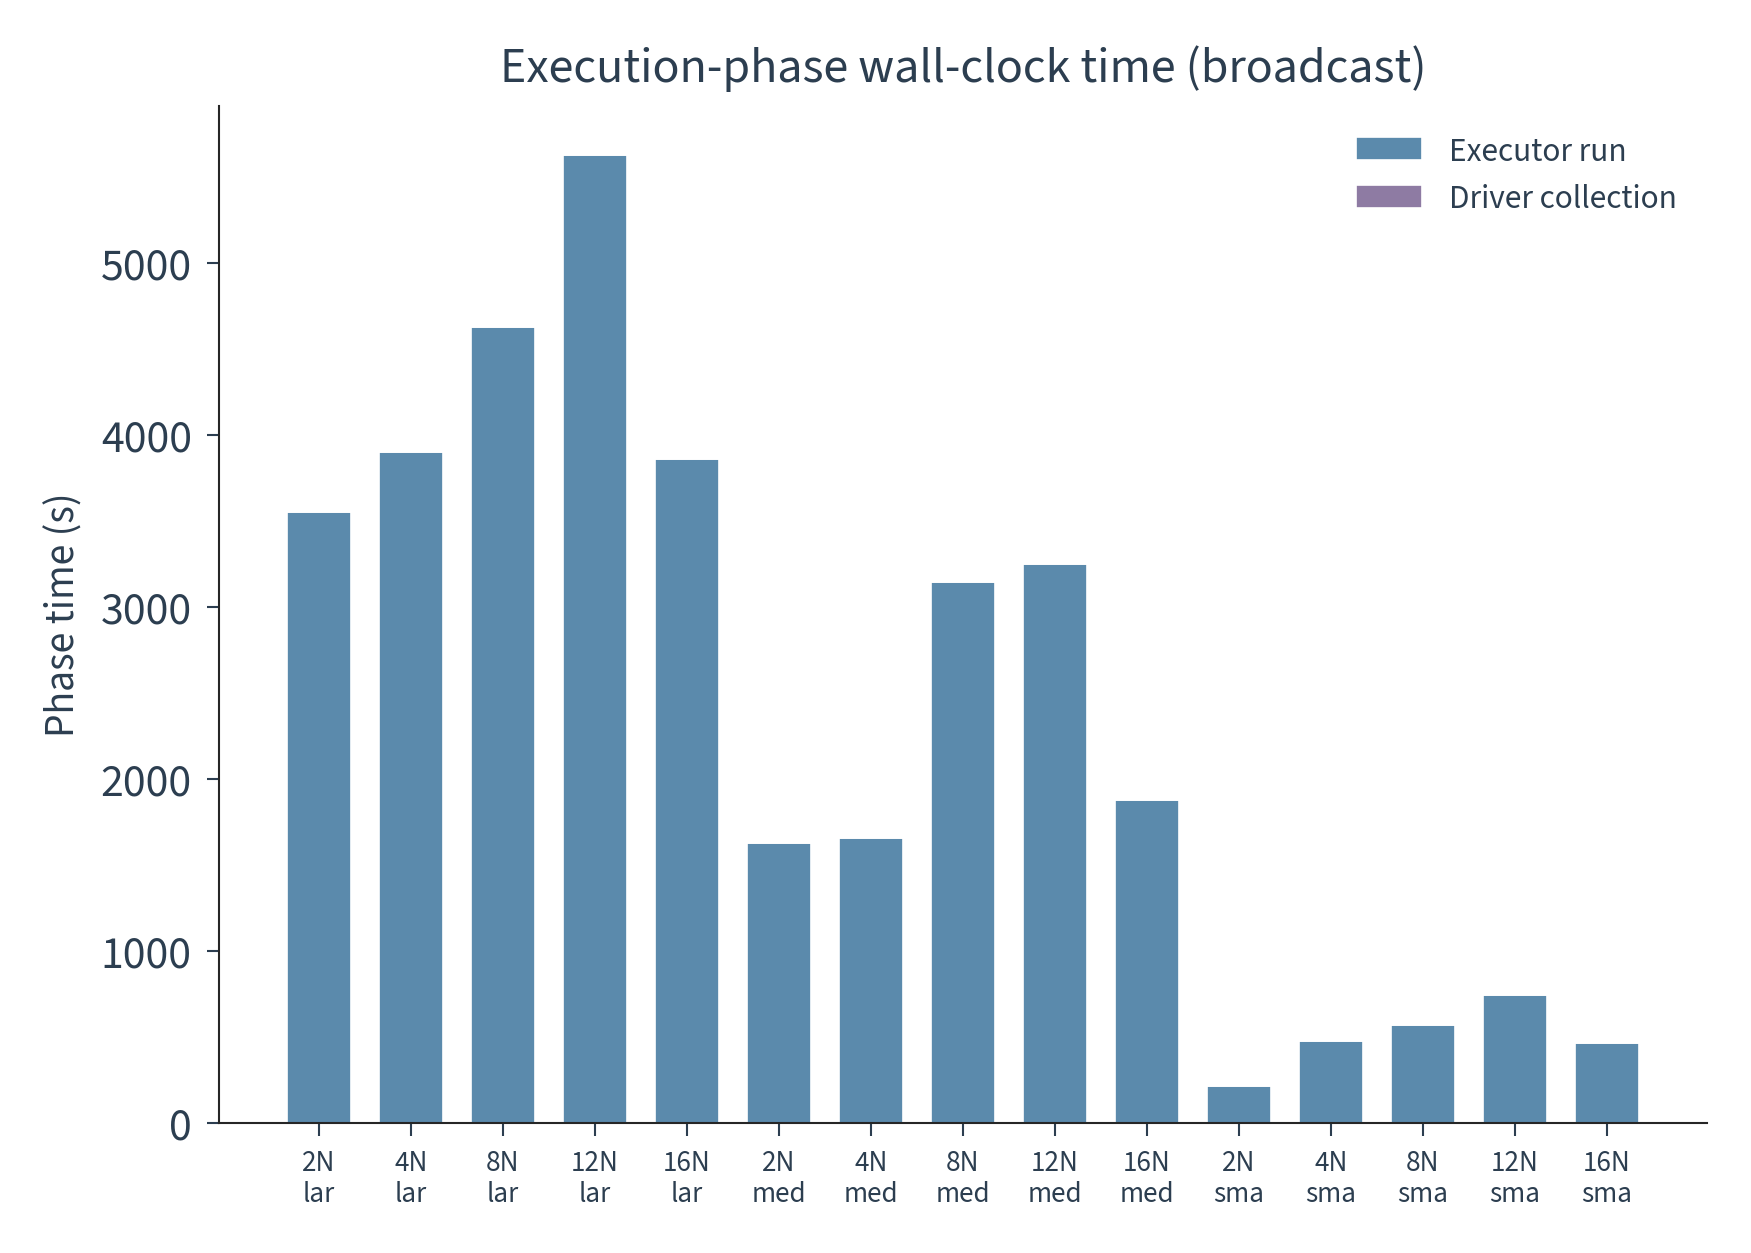
\includegraphics[valign=t, width=0.45\textwidth]{Chapters/06-results/sub-chapters/figures/06-distributed-phase-time.png}}%
    \hfill
    \subfloat[Shuffle bytes.\label{fig:distributed-shuffle-bytes}]{%
        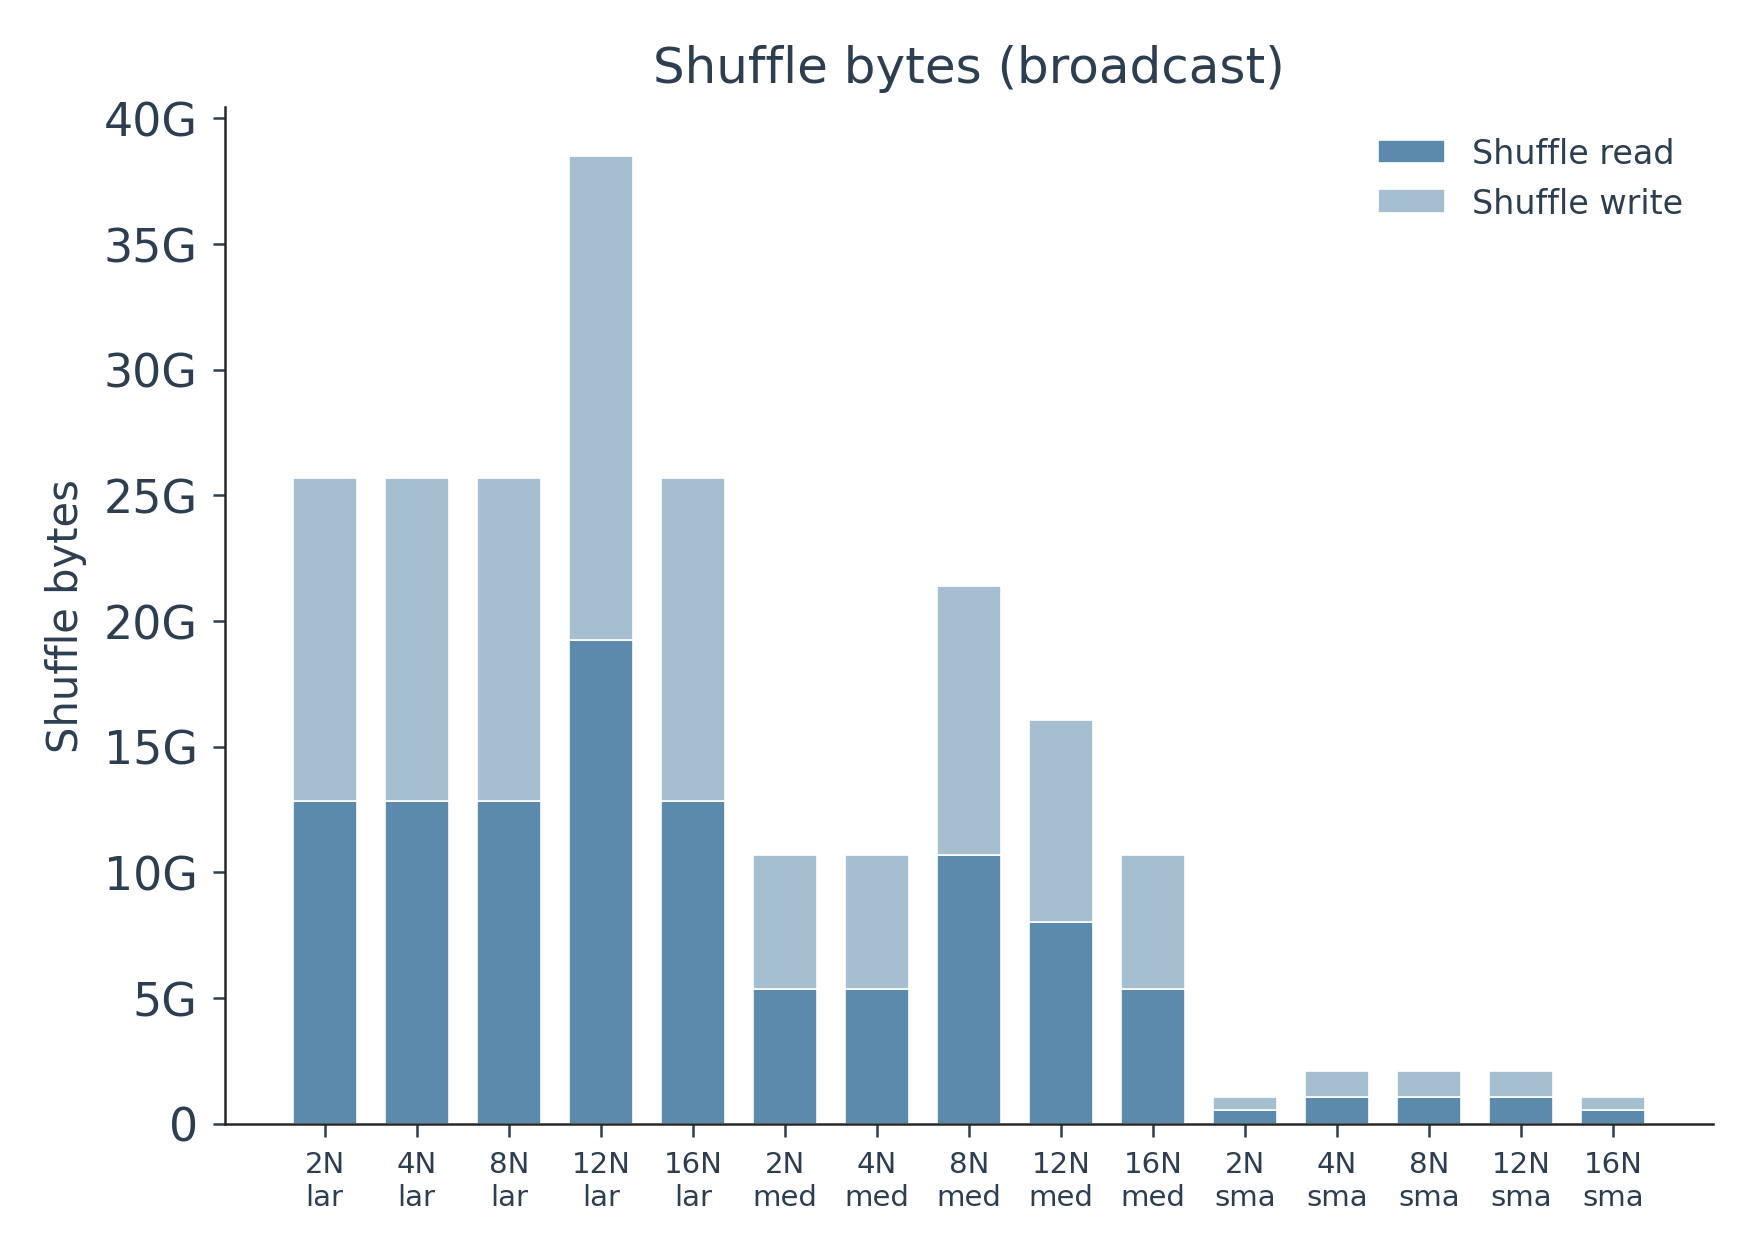
\includegraphics[valign=t, width=0.45\textwidth]{Chapters/06-results/sub-chapters/figures/06-distributed-shuffle-bytes.png}}%
    \caption[Execution-phase breakdown of the distributed join]{Decomposition of
    the distributed join across the three instrumented phases of the distributed
    lifecycle -- executor read time, shuffle, and driver collection (the last
    recovered as the clamped wall-clock residual). Panel~(a) stacks wall-clock
    time by phase against worker count; panel~(b) shows the corresponding shuffle
    bytes. Phase colour uses the thesis palette.}
    \label{fig:distributed-execution-phase-breakdown}
\end{figure}

\subsection{Operational cost and the cost-time tradeoff}
\label{results:distributed-join-and-scaling:operational-cost-and-the-cost-time-tradeoff}

% TODO (prose): factual readout only of cost vs. time across worker counts, and
% which points lie on the frontier. Refer to
% Figure~\ref{fig:distributed-cost-time-pareto} and
% Table~\ref{tab:distributed-join-descriptive-statistics}. No interpretation.

\begin{figure}[H]
    \centering
    % WHAT IT SHOWS: cost-time Pareto scatter. One point per worker count
    %   {2, 4, 8, 12, 16} in (wall-clock time, operational cost) space, a separate
    %   series for broadcast and partitioned; the non-dominated points are joined
    %   to trace the Pareto frontier.
    % CAPTION MUST STATE: the two axes (time, cost); that each point is one worker
    %   count; the two strategies; and that the frontier is the non-dominated set.
    % DESCRIPTIVE ONLY: report which points are non-dominated; no interpretation.
    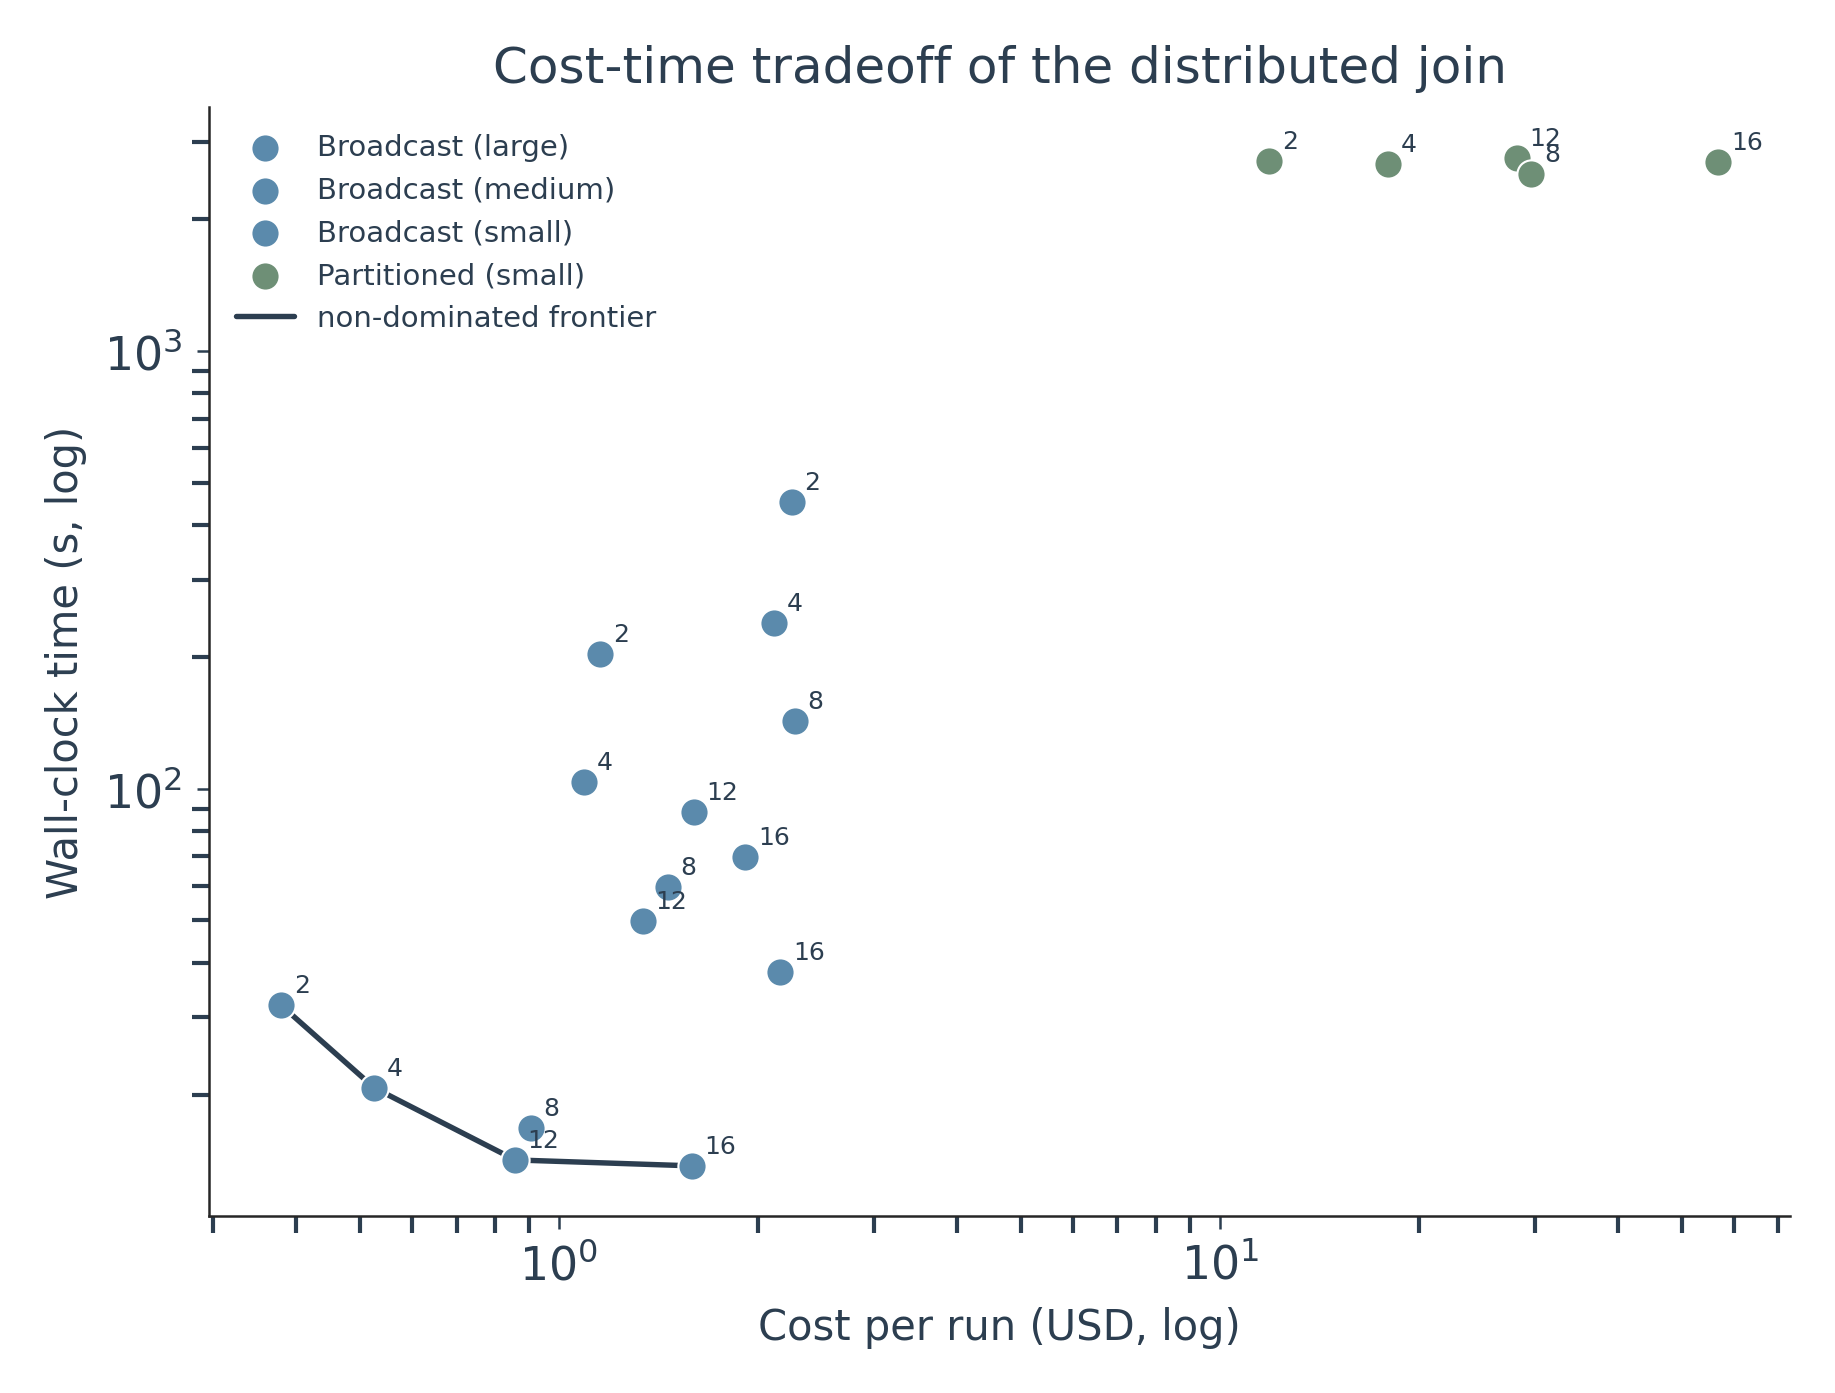
\includegraphics[width=0.75\textwidth]{Chapters/06-results/sub-chapters/figures/06-distributed-cost-time-pareto.png}
    \caption[Cost-time tradeoff of the distributed join]{Operational cost against
    wall-clock time for the distributed join, with one point per worker count and
    a separate series for each join strategy. The non-dominated points trace the
    cost-time Pareto frontier. Series colour encodes join strategy using the
    thesis palette.}
    \label{fig:distributed-cost-time-pareto}
\end{figure}

\begin{table}[H]
    \centering
    % WHAT IT SHOWS (supplementary): descriptive statistics of the distributed
    %   join per (configuration x size tier x worker count): achieved n, minimum
    %   estimator, CI half-width, dispersion, and the cost terms.
    % CAPTION MUST STATE: the columns and units; the estimator and CI method.
    % DATA: leave every data row commented out -- do NOT invent numbers.
    % NOTE: if the grid overflows one page, convert table -> longtable.
    \footnotesize
    \setlength{\tabcolsep}{6pt}
    \renewcommand{\arraystretch}{1.2}
    \begin{tabular}{@{}l l r r r r r@{}}
        \toprule
        \textbf{Tier} & \textbf{Strategy} & \textbf{Workers} & \textbf{Achieved $n$} & \textbf{Min.\ (\si{\second})} & \textbf{CI half-width} & \textbf{Cost (USD)} \\
        \midrule
        % TODO: one row per (tier x strategy x worker count). Example shape only,
        % no real numbers -- fill from run metadata:
        % Large & Broadcast   & 2  & <n> & <min> & <hw> & <cost> \\
        % Large & Partitioned & 16 & <n> & <min> & <hw> & <cost> \\
        % ...
        \bottomrule
    \end{tabular}
    \caption[Distributed join descriptive statistics]{Descriptive statistics of the
    distributed join for each size tier, join strategy, and worker count: the
    achieved iteration count, the minimum-estimator elapsed time, its bootstrap
    confidence-interval half-width, and the associated operational cost.}
    \label{tab:distributed-join-descriptive-statistics}
\end{table}

\section{Consistency of winners (RQ3)}
\label{results:consistency-of-winners}

% TODO: section-opening placeholder. Present which configuration wins on each
% outcome dimension across all workload patterns and size tiers. Refer to
% Figure~\ref{fig:winners-matrix}. Results only.

\begin{figure}[H]
    \centering
    % TODO: winners matrix / heatmap. Rows = workload pattern x size tier;
    % columns = outcome dimension (data transferred, wall-clock time, operational
    % cost). Each cell coloured by the winning configuration using the thesis
    % palette (\texttt{thesisteal} DuckDB, \texttt{thesiscoral} Apache Sedona,
    % \texttt{thesissteel} PostGIS, \texttt{thesisamber} GeoPandas/Shapefile).
    % Leave the large-tier Shapefile rows free of any Shapefile-winner marking
    % (small tier only); do not imply a missing cell.
    \caption[Consistency of winners across dimensions]{Winning configuration for
    every workload pattern and size tier (rows) on each outcome dimension (columns:
    data transferred, wall-clock time, operational cost). Cell colour encodes the
    winning configuration using the thesis palette.}
    \label{fig:winners-matrix}
\end{figure}

% TODO: closing paragraph placeholder. Give an interpretation-free recap of the
% results presented in this chapter -- which orderings held and where they
% diverged -- without explaining why. All interpretation is deferred to the
% Discussion (Chapter~\ref{ch:discussion}). Do not add a separate summary section.

